%%%%%%%%%%%%%%%%%%%%%%%%%%%%%%%%%%%%%%%%%%%%%%%%%%%%%%%%%%%%%%%%%%%%%
%% This is a "template" model document for submission to the
%% American Chemical Society (ACS).
%%
%% The guidance here contains information about how you may wish to
%% modify it to match the requirements of various ACS journals. The
%% ACS do *not* typeset accepted articles using LaTeX, so there is
%% no specific class required.
%%
%% This template deliberately does *not* seek to reproduce
%% the layout of the typeset journal: this is explicitly not
%% required by the ACS for LaTeX submissions.
%%
%% Please report any issues with the template at
%% https://github.com/josephwright/acs-template/issues
%%
%% Released under the Creative Commons 0 license
%% https://creativecommons.org/public-domain/cc0/
%% 
%% Copyight (c) 2025 Joseph Wright
%%%%%%%%%%%%%%%%%%%%%%%%%%%%%%%%%%%%%%%%%%%%%%%%%%%%%%%%%%%%%%%%%%%%%
\documentclass[letterpaper]{article}

%%%%%%%%%%%%%%%%%%%%%%%%%%%%%%%%%%%%%%%%%%%%%%%%%%%%%%%%%%%%%%%%%%%%%
%% Font setup - delete if you are using LuaLaTeX
%%%%%%%%%%%%%%%%%%%%%%%%%%%%%%%%%%%%%%%%%%%%%%%%%%%%%%%%%%%%%%%%%%%%%
\usepackage[T1]{fontenc}

%%%%%%%%%%%%%%%%%%%%%%%%%%%%%%%%%%%%%%%%%%%%%%%%%%%%%%%%%%%%%%%%%%%%%
%% Adjust the margins and allow for line spacing
%%%%%%%%%%%%%%%%%%%%%%%%%%%%%%%%%%%%%%%%%%%%%%%%%%%%%%%%%%%%%%%%%%%%%
\usepackage{geometry}
\geometry{margin = 1in}
\usepackage{setspace}

%%%%%%%%%%%%%%%%%%%%%%%%%%%%%%%%%%%%%%%%%%%%%%%%%%%%%%%%%%%%%%%%%%%%%
%% Reference support
%%
%% The recommended method for producing the reference section is
%% to use biblatex. If you wish to use a classical BibTeX
%% approach, this is easiest to achieve using the achemso package.
%% In that case, you should remove the biblatex lines.
%%%%%%%%%%%%%%%%%%%%%%%%%%%%%%%%%%%%%%%%%%%%%%%%%%%%%%%%%%%%%%%%%%%%%
% You can adjust the printing of DOI, article title, etc. using
% package options, e.g. "doi = true"; see the biblatex manual for
% details of adjusting the number of authors printed, e.g.
% "maxnames = 15" to print no more than 15 authors.
\usepackage[style = chem-acs]{biblatex}
\addbibresource{acs-template.bib}
% If you are using classical BibTeX, remove the above lines and 
% uncomment:
%\usepackage{achemso}

%%%%%%%%%%%%%%%%%%%%%%%%%%%%%%%%%%%%%%%%%%%%%%%%%%%%%%%%%%%%%%%%%%%%%
%% Graphic inclusion and scheme and chart support
%%%%%%%%%%%%%%%%%%%%%%%%%%%%%%%%%%%%%%%%%%%%%%%%%%%%%%%%%%%%%%%%%%%%%
\usepackage{graphicx}
\usepackage{float}
\newfloat{scheme}{htbp}{los}
\floatname{scheme}{Scheme}
\floatname{chart}{Chart}
\newfloat{graph}{htbp}{loh}

%%%%%%%%%%%%%%%%%%%%%%%%%%%%%%%%%%%%%%%%%%%%%%%%%%%%%%%%%%%%%%%%%%%%%
%% Common support packages
%%%%%%%%%%%%%%%%%%%%%%%%%%%%%%%%%%%%%%%%%%%%%%%%%%%%%%%%%%%%%%%%%%%%%
\usepackage{chemformula} % Formulas using \ch{}
% or
\usepackage[version = 4]{mhchem} % Formulas using \ce{}

%%%%%%%%%%%%%%%%%%%%%%%%%%%%%%%%%%%%%%%%%%%%%%%%%%%%%%%%%%%%%%%%%%%%%
%% Many journals require that sections are unnumbered: this 
%% is activated here
%%%%%%%%%%%%%%%%%%%%%%%%%%%%%%%%%%%%%%%%%%%%%%%%%%%%%%%%%%%%%%%%%%%%%
\setcounter{secnumdepth}{-1}

%%%%%%%%%%%%%%%%%%%%%%%%%%%%%%%%%%%%%%%%%%%%%%%%%%%%%%%%%%%%%%%%%%%%%
%% Place any additional macros here.  Please use \newcommand* where
%% possible, and avoid layout-changing macros (which are not used
%% when typesetting).
%%%%%%%%%%%%%%%%%%%%%%%%%%%%%%%%%%%%%%%%%%%%%%%%%%%%%%%%%%%%%%%%%%%%%
\newcommand*\mycommand[1]{\texttt{\emph{#1}}}

%%%%%%%%%%%%%%%%%%%%%%%%%%%%%%%%%%%%%%%%%%%%%%%%%%%%%%%%%%%%%%%%%%%%%
%% Author and title data:
%% the authblk package is currently the simplest way to provide this
%%%%%%%%%%%%%%%%%%%%%%%%%%%%%%%%%%%%%%%%%%%%%%%%%%%%%%%%%%%%%%%%%%%%%
\usepackage{authblk}
\author[1]{Andrew N. Other}
\author[1]{Fred T. Secondauthor}
\author[1]{I. Ken Groupleader*}
\affil[1]{Department of Chemistry, Unknown University, Unknown Town}
\author[2]{Susanne K. Laborator}
\affil[2]{Lead Discovery, BigPharma, Big Town, USA}
\author[1]{Kay T. Finally}

\title{A ``template'' model document for submission to the
  American Chemical Society (ACS)}
% Use the \date command for email address(s) of corresponding authors
\date{*Email: i.k.groupleader@unknown.uu}

\begin{document}

\maketitle

\begin{abstract}
  This is an example document for creating \LaTeX{} submissions to the American
  Chemical Society (ACS) for publication. As ACS does not use \LaTeX{} for
  typesetting accepted manuscripts, this template does not seek to
  reproduce the appearance of a published paper.
\end{abstract}

\section*{Keywords}

Some journals require keywords: these normally should be given immediately
after the abstract.

\section*{Abbreviations}

Some journals require a list of abbreviations: these normally should be given
immediately after the keyswords (if required).

%%%%%%%%%%%%%%%%%%%%%%%%%%%%%%%%%%%%%%%%%%%%%%%%%%%%%%%%%%%%%%%%%%%%%
%% Start the main part of the manuscript here.
%%%%%%%%%%%%%%%%%%%%%%%%%%%%%%%%%%%%%%%%%%%%%%%%%%%%%%%%%%%%%%%%%%%%%
\section{Introduction}
\label{sec:introduction}

Conformer generators provide candidate three-dimensional geometries for
molecular modeling when the required structure is not known in advance.
Molecular shape comparison and pharmacophore screening use these geometries
to compare spatial arrangements of atoms or interaction features, while
docking searches for ligand geometries compatible with a binding site.
Even docking methods that allow ligand flexibility may sample only some
internal degrees of freedom, making their results dependent on the supplied
conformations.\cite{mcnutt2023conformers} Experimentally determined
protein--ligand structures provide reference geometries for assessing whether
a generated ensemble contains a bioactive conformation.

Previous work has established that ensemble construction affects the usefulness
of generated conformations. McNutt et al.\ examined RDKit ETKDG and the deep
generative model DMCG, varying ensemble size, conformer selection, and energy
minimization, and evaluated bioactive conformation recovery, pharmacophore
screening, and docking.\cite{mcnutt2023conformers} That study connected
generation choices to application performance using a focused comparison of
two generators. Selecting among the wider range of available generators
requires a complementary comparison of their ability to recover observed
bound geometries while preserving molecular identity and local geometric
plausibility under specified sampling allowances.

The available methods span substantially different sampling procedures.
Distance geometry combines molecular connectivity with geometric constraints
and experimental torsional preferences.\cite{wang2020etkdg} Learned
approaches include diffusion over torsions, continuous conformer fields,
and molecular language representations.\cite{jing2022torsional,wang2024mcf,liu2025nextmol}
LoQI and its associated ChEMBL3D ensembles emphasize low-energy
structures,\cite{nikitin2025loqi} while FlowR provides another learned
approach to coordinate generation.\cite{cremer2025flowr} Their different
representations, refinement procedures, and filtering policies make it
necessary to evaluate the resulting ensembles against common structural
criteria. Performance of one learned generator cannot establish the
suitability of these other methods for recovering bioactive conformations.

Here, we define an evaluation protocol for selecting generators of ensembles
intended to recover bioactive conformations. A successful ensemble must
contain at least one conformer that preserves the requested molecular
identity, passes intramolecular plausibility checks, and lies within
0.75~\AA{} heavy-atom root mean square deviation (RMSD) of the experimental
geometry after alignment. PoseBusters supplies the identity and plausibility
checks.\cite{buttenschoen2024posebusters} We compare two candidate allowances:
the stored ChEMBL3D count for each ligand and 1,000 conformers per ligand.
These allowances apply before filtering; retained counts are reported
alongside recovery. Geometric diversity is evaluated as a possible indicator
of recovery, rather than imposed as a minimum requirement: a diverse pool
need not contain a close match to the bound geometry.

Our main comparison includes four classical generation pipelines and six
learned generators: LoQI, Torsional Diffusion, Molecular Conformer Fields,
NExT-Mol, FlowR, and an autoregressive Qwen model. This broader method panel
extends the focused RDKit--DMCG comparison to assess which evaluated
generators satisfy the same recovery criterion under the specified validity
and sampling conditions. The primary cohort comprises 94 CASF-2016 ligand
entries matched to ChEMBL3D; its stored ensembles provide an additional
comparison.\cite{su2019casf,nikitin2025loqi} Analyses by molecular size and
flexibility identify where each generator fails to recover the bound
geometry. Results for a larger reference cohort are provided in the
Supporting Information.

Recovery of one bound structure does not describe how often a generator
samples near observed conformations or whether it covers other observed
geometries of the same molecule. A separate exploratory panel of 23 druglike
molecules with multiple experimental references distinguishes reference
coverage from the fraction of generated samples close to those references.
Together, these evaluations assess recovery and sample concentration for
generator selection. The multi-reference comparison remains subject to
differences in filtering and failure handling described in Methods.
The study evaluates structural recovery rather than downstream screening or
docking performance, and the experimental references are not assumed to
exhaust the accessible conformations of a molecule.
% AUTHOR: resolve dataset provenance, checkpoint selection and training overlap
% audits before claiming performance on unseen molecules or broad generalization.
 

% Benchmark Methods and Results; front and end matter retain template examples.
% Revised 28 September 2026 using the corrected 24 September snapshot.
% Read METHODS_NOTES.md before submission. In particular, training and inference
% metadata and the provenance of the larger reference cohort remain incomplete.
\section{Methods}
\label{sec:methods}

\subsection{Benchmark datasets and molecular identity}

We evaluated conformer ensembles against experimental ligand geometries using
two complementary settings: recovery of one bound conformation per
protein--ligand complex and coverage of several observed conformations of the
same molecule. The CASF-2016 core and larger reference ligand collections
are denoted core and ref, respectively.\cite{su2019casf}
% AUTHOR: establish the exact source release and construction of CASF16_REF;
% the CASF citation alone does not document that local collection.
Ligands were matched to ChEMBL3D by exact canonical, heavy-atom isomeric SMILES.
ChEMBL3D provided molecular topologies and a separate computed conformer
ensemble for comparison.\cite{nikitin2025loqi}
Entries were retained when the ligand could be parsed, a matching topology was
available, and at least one eligible torsion was identified by the SMARTS
pattern \texttt{[!\$(*\#*)\&!D1]-!@[!\$(*\#*)\&!D1]}.
This torsion eligibility rule differs from the descriptor for the number of rotatable bonds used to stratify the results.

We resolved stereoisomers within each ChEMBL3D parent record using isomeric
SMILES and the tetrahedral and double-bond stereochemistry layers of InChI.
The selected topology record was retained in the mapping, and stored
coordinates were filtered to the matching stereoisomer. Thus, both the
reference ensemble and its conformer count were specific to the mapped
stereoisomer. The resulting core cohort contained 94 complex entries and 94
ChEMBL parent compounds; ref contained 1,236 entries and 1,042 parent compounds.
The cohorts shared no complex identifiers but included 17 common parent
compounds. We retained separate complex entries because they provide separate
experimental reference geometries, while accounting for repeated compounds
in the uncertainty analysis.

The second setting used a curated set of 23 druglike molecules with 2,450
stored experimental reference conformations in total, ranging from 23 to 716
per molecule. We used the supplied molecular identities and reference
coordinates without treating the frequency of a structure in this collection
as an equilibrium population. The collection is an incomplete set of observed conformations.
% AUTHOR: add the dataset release, selection and structure-cleaning procedure,
% and original dataset citation after verifying the supplied collection's lineage.

\subsection{Conformer generators}

The main comparison included four classical generators, five external learned
generators, and one representative Qwen checkpoint. The classical
generators comprised RDKit distance geometry and torsion perturbation, each
with and without energy minimization. RDKit conformers were generated with
ETKDGv3 from a molecular topology without coordinates, using random starting coordinates,
enforced chirality, and no RMSD pruning.\cite{wang2020etkdg}
The minimized variant applied MMFF94s for up to 500 iterations. Structures
that reached the iteration limit were retained if the optimization returned
normally; convergence was not required. The two variants used independently
sampled pools.

Torsion perturbation started from the matched ChEMBL3D topology's stored
geometry. In each trial, every eligible torsion received an independent
uniform angular displacement between $-120^{\circ}$ and $120^{\circ}$.
Candidates were rejected if a nonbonded heavy-atom distance was below 0.7
times its distance-geometry lower bound; bonded and 1,3 pairs were excluded
from this check. The minimized variant additionally applied MMFF94s and
repeated the clash check. Candidate generation continued toward the requested
pool size before the common validity filter was applied.

The external methods were LoQI,\cite{nikitin2025loqi} Torsional
Diffusion,\cite{jing2022torsional} Molecular Conformer Fields (MCF,
drugs-L),\cite{wang2024mcf} NExT-Mol
(DMT-L),\cite{liu2025nextmol} and FLOWR.root, referred to here as
FlowR.\cite{cremer2025flowr} We evaluated their saved conformer outputs through
the benchmark adapters. FlowR used the v2.2 checkpoint for generation of ligands alone, with the
input atom and bond graph fixed during coordinate generation. Its adapter
included up to 200 steps of force-field cleanup, using MMFF with UFF as a
fallback, and stereochemistry checks; mirror reflection was allowed when it
restored the requested stereoisomer. Remaining stereochemical mismatches
were rejected. Consequently, an ensemble labeled raw in the benchmark can
already include preprocessing specific to its generator.

The Qwen generator produced conformations autoregressively from molecular
SMILES. The main analysis used the model with 1.7 billion parameters and finite
scalar quantization (FSQ), evaluated at pretraining step 47,023. The
comparison with multiple experimental references used the same representative Qwen checkpoint and the five external methods.
Overlap of the training set with the benchmark molecules has not been established
by a common audit.
% AUTHOR: document the checkpoint-selection rule, including any use of these
% benchmark outcomes. Supply training datasets/splits, representation and decoder
% details, inference settings, checkpoint hashes, and Qwen/FSQ citations.

\subsection{Ensemble sizes and validity filtering}

The main CASF comparison used two candidate targets per ligand, both defined
before the common validity filter. The ChEMBL-count tier used a target equal
to the stored ChEMBL3D conformer count for the mapped stereoisomer, while the
fixed tier used a target of 1,000 conformers. The ChEMBL-count tier was sampled
without replacement from each available candidate pool. Subsets were capped
at the available pool size and then subjected to the same validity filter.
The subsets were drawn from existing outputs, without separate generation
runs or matching of computational cost.
The launcher for classical generation used base seed 42; the common
procedure for assembling ensembles from saved pools used base seed 1729.
Seeds for each molecule and method were derived from these values.

We applied PoseBusters to assess molecular identity and intramolecular
plausibility.\cite{buttenschoen2024posebusters} The configured checks covered
loading, sanitization, InChI conversion, connectivity, radicals, molecular
formula, bond connectivity, tetrahedral and double-bond stereochemistry,
bond lengths and angles, internal clashes, planarity, and energy ratio.
The distance-geometry tolerances were 0.25 for bond lengths and angles and
0.3 for clashes, with hydrogens excluded from these distance checks.
Planarity tolerance was 0.25~\AA{} for the specified aromatic rings and
trigonal carbon--carbon double-bond groups. The threshold for the energy ratio was
100, using a reference ensemble of 50 conformations. No checks of contacts with the protein were included.

A conformer passed only if all configured Boolean checks passed. Generated
CASF ensembles were checked against the matched ChEMBL3D molecular reference;
the stored ChEMBL3D comparison ensembles were checked against the CASF ligand.
The same pass mask was applied to the full candidate pool and its sampled
subsets. Rejected conformers were not replaced after filtering. Retained
ensemble sizes and numbers of generation attempts could differ between
methods at the same candidate target.
ChEMBL3D was evaluated as a finite stored ensemble, with a cap of 2,000 conformers for the designated large reference entry, 1tlp, when necessary.

\subsection{Conformational recovery and diversity}

CASF recovery was evaluated on conformers that passed PoseBusters, using the
experimental ligand geometry as the target. We removed hydrogens and used
RDKit's symmetry-aware \texttt{GetBestRMS} alignment. If this alignment raised
an exception, the CASF implementation attempted \texttt{AlignMol} with atoms matched by their indices. An unresolved, nonfinite RMSD caused analysis of
that ensemble to fail.

For each ligand, we calculated the minimum and median RMSD over the retained
ensemble. Hit@$\delta$ was one when at least one conformer had RMSD
$\leq\delta$, and zero otherwise, at thresholds of 0.25, 0.5, 0.75, and
2.0~\AA. We used 0.75~\AA{} as the principal recovery cutoff
and the remaining thresholds to assess sensitivity. Cohort hit rates used all mapped entries as the denominator,
including empty or missing outputs as misses. We averaged the minimum RMSD, ensemble median RMSD, and diversity
measures only over entries with defined values.

We measured geometric diversity by greedy clustering of the retained
conformers at a principal heavy-atom RMSD threshold of 1.0~\AA{},
with additional radii of 0.5 and 2.0~\AA{} for sensitivity analysis. Conformers were visited
in stored order and assigned to the nearest existing cluster representative
if their RMSD was below the threshold; otherwise, a new cluster was created.
We reported the mean number of clusters across measurable ensembles.
This measure describes geometric spread and depends on ensemble size
and clustering order.

\subsection{Coverage of multiple experimental conformations}

For each druglike molecule, we compared the supplied generated pool with all
of its experimental references using aligned heavy-atom RMSD. Recall
coverage (COV-R) was the fraction of reference conformations with a generated
neighbor below 0.75~\AA. Precision coverage (COV-P) was the fraction of
generated conformations with a reference neighbor below the same threshold.
Matching distance MAT-R was the mean RMSD from each reference to its
nearest generated conformer; MAT-P was the mean RMSD from each generated
conformer to its nearest reference. Unlike CASF Hit@$\delta$, coverage used a strict inequality.
We averaged each metric equally across molecules. COV-P measures proximity
to the available observations; a low value does not establish that the
remaining conformers are physically inaccessible.

These coverage calculations used the supplied generated pools without a
common PoseBusters filter. Validity was assessed separately. The imported
Qwen evaluator counted reference or generated conformations with no finite
RMSD match as coverage misses, whereas the local evaluator for external methods
excluded them from the corresponding coverage denominator. Both omitted
undefined distances to the nearest match from MAT. Differences in filtering
and failure handling limit the comparability of these coverage estimates.

\subsection{Statistical analysis}

We calculated paired differences in recovery and coverage on the same
complex entries or druglike molecules. For CASF, 95\% confidence intervals were obtained from
3,000 bootstrap resamples of ChEMBL parent compounds, retaining all complex
entries belonging to each sampled compound. Each resample used the mean
over its complex entries, preserving equal weighting of entries while
accounting for repeated compounds. Missing hits were assigned zero.
For druglike method differences, we used 10,000 paired resamples of the
23 molecules. Intervals for each method's mean COV-R and COV-P
(Figure~\ref{fig:druglike}A) used 10,000 resamples of the same molecules.

Intervals were the 2.5th and 97.5th percentiles of the bootstrap distribution,
using a NumPy random generator initialized with seed 20260924. These
intervals quantify uncertainty from resampling the evaluated molecules.
They do not include variation across independent generation or training runs.
% Provenance: CASF/drug paired intervals were calculated in
% docs/publication_analysis_2026_09_24.py and archived in paired_cluster_bootstrap.csv
% and druglike_paired.csv. Figure 4 marginal intervals were added by
% manuscript/build_figures.py, not provided by the public dashboard; see
% figure-data/drug_coverage_intervals.csv.

As an overlap sensitivity analysis, we repeated ref comparisons after
excluding the 17 parent compounds also present in core, leaving 1,189
complex entries from 1,025 compounds. Exploratory size analyses used
counts of heavy atoms from the experimental ligand after removing hydrogens, grouped
as fewer than 20, 20--29, 30--39, and at least 40 atoms. Flexibility analyses
used RDKit counts of rotatable bonds from that same reference, grouped as 0--3,
4--6, 7--8, and at least 9. These descriptors from the experimental reference assigned each
entry to the same group for every generator. Stratum hit rates included all
mapped entries in the group, with missing outputs counted as misses.
These descriptive analyses did not adjust size effects for flexibility or
chemical class. Confidence intervals were not adjusted for multiple
comparisons or checkpoint selection.


% Results draft; see RESULTS_NOTES.md for evidence and unfinished analyses.
% Revised 28 September 2026 following the annotated PDF comments.
% Numerical sources: publication_tables_2026_09_24 and size strata of 28 September.
% Core counts independently checked against the public-release per_ligand_long
% records; see figure-data/core-recovery-audit.csv and core-recovery-counts.csv.
\section{Results}
\label{sec:results}
% Figures transferred from the working Results; sources are in results-data/.
\newcommand{\diversityfigure}{%
\begin{figure}[htbp]
\centering
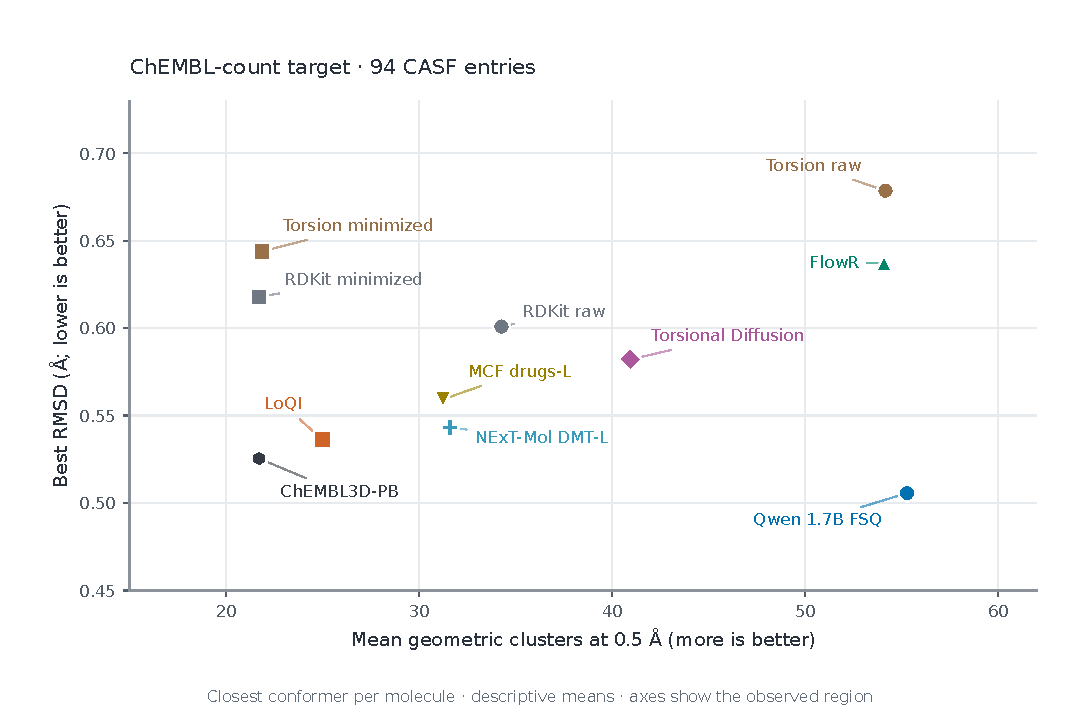
\includegraphics[width=\linewidth]{figures/figure-2-diversity-recovery.pdf}
\caption{Geometric diversity and experimental recovery at the ChEMBL-count target. Each point represents one evaluated pipeline or the stored ChEMBL3D-PB ensemble. Clustering uses a 1.0 \AA{} radius, whereas recovery requires at least one retained conformer at RMSD $\leq$ 0.75 \AA{}. Cluster counts are averaged over defined measurements; recovery uses all 94 entries, including failures. Retained ensemble sizes differ despite matched candidate targets. These are descriptive method summaries, not a causal analysis of diversity.}
\label{fig:diversity-recovery}
\end{figure}}

\newcommand{\recoveryfigure}{%
\begin{figure}[htbp]
\centering
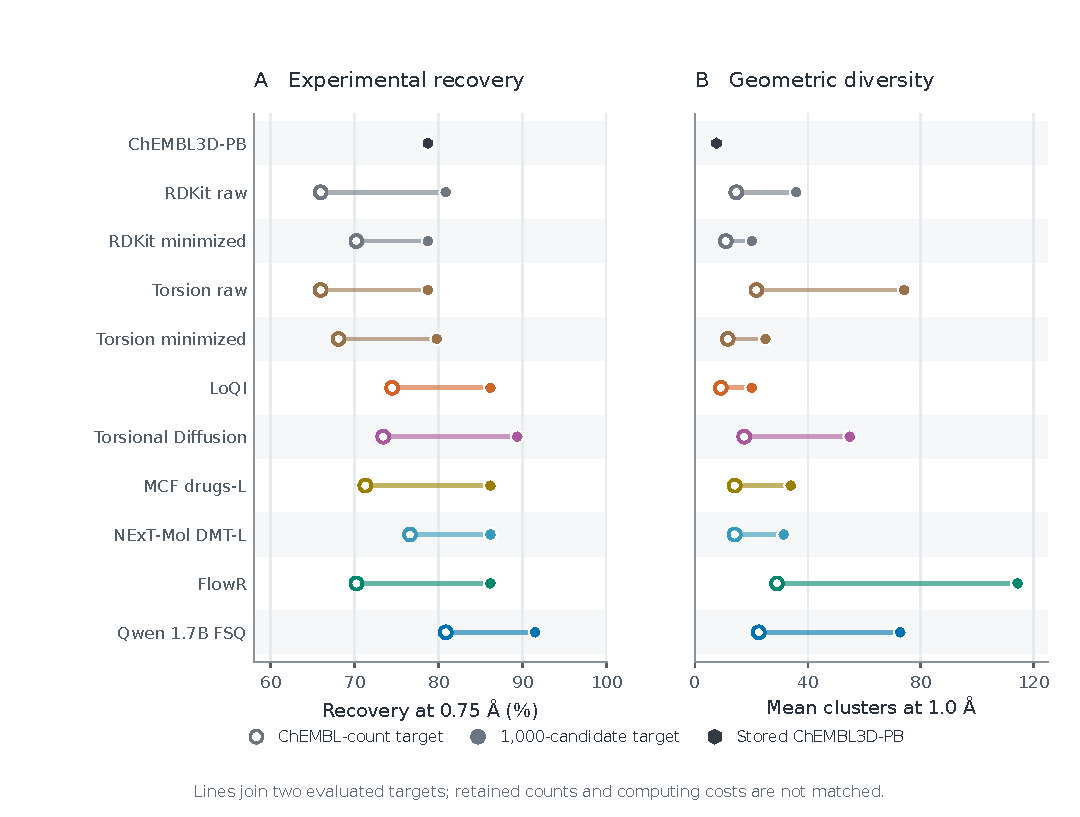
\includegraphics[width=\linewidth]{figures/figure-3-sampling-budget.pdf}
\caption{Recovery and diversity at the two candidate targets. Open circles denote the ChEMBL-count target and filled circles the 1,000-candidate target. Each row follows the same method between the two targets. The stored ChEMBL3D-PB ensemble is shown once as a hexagon. Recovery uses all 94 CASF entries; cluster means use defined measurements. Lines connect observed endpoints and do not represent random-subsampling curves or intermediate measurements. Targets precede PoseBusters filtering; retained counts are given in Table~\ref{tab:recovery}.}
\label{fig:recovery}
\end{figure}}

\newcommand{\sizefigure}{%
\begin{figure}[htbp]
\centering
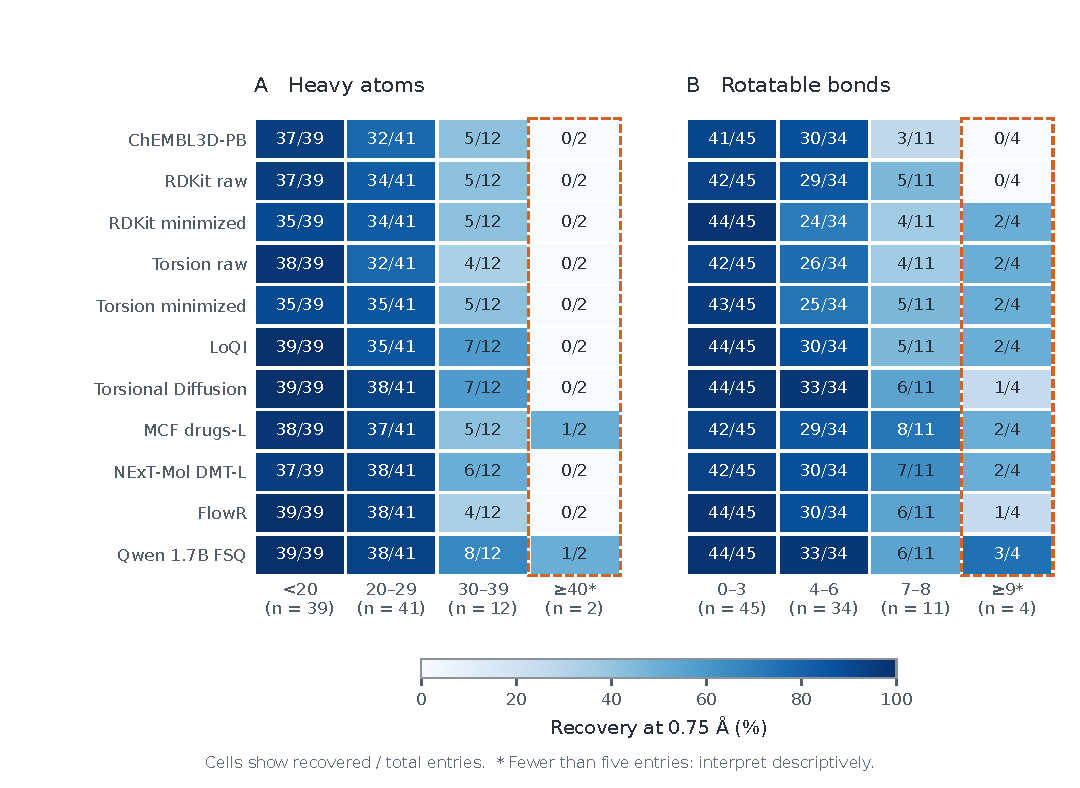
\includegraphics[width=\linewidth]{figures/figure-4-size-flexibility.pdf}
\caption{Recovery by molecular size and flexibility. Generated methods use the 1,000-candidate target; ChEMBL3D-PB uses its stored ensemble. Every cell gives recovered/total CASF entries, with the color indicating the corresponding percentage. Dashed outlines mark groups with fewer than five entries. Heavy-atom and rotatable-bond groups are analyzed separately and do not isolate independent effects of size and flexibility. Sparse groups cannot establish stable method rankings.}
\label{fig:size}
\end{figure}}

\newcommand{\drugfigure}{%
\begin{figure}[htbp]
\centering
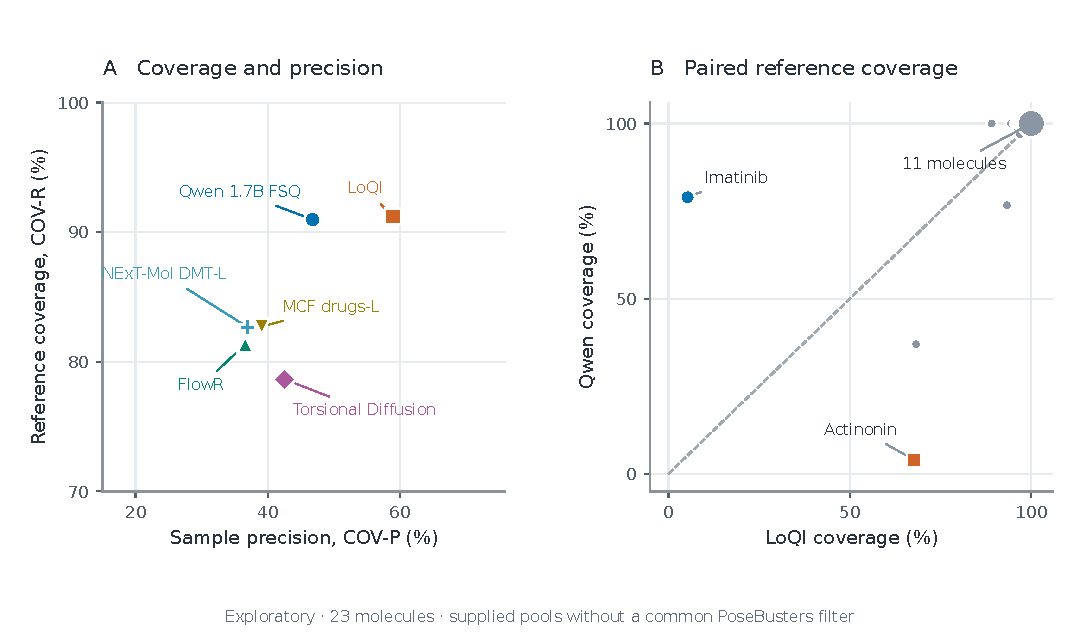
\includegraphics[width=\linewidth]{figures/figure-5-multiple-references.pdf}
\caption{Coverage of multiple bound references and precision relative to those observations. (A) Molecule-averaged COV-R and COV-P for six learned generators, using the existing strict RMSD $<$ 0.75 \AA{} criterion. Axes are restricted to the observed range for readability. (B) Paired reference coverage for Qwen and LoQI across all 23 molecules; the diagonal denotes equal coverage. Coincident points are grouped and labeled, including 11 molecules with complete coverage by both methods. Imatinib and actinonin are the examples retained from the earlier draft. These are descriptive supplied-pool results with differing RMSD-failure conventions, not a comparison after common validity filtering. No uncertainty intervals are shown; paired uncertainty is documented in the archived findings.}
\label{fig:druglike}
\end{figure}}


\subsection{Recovery depended on the sampling allowance}

We compared generators on the core cohort of 94 ligands by counting a ligand
as recovered when at least one conformer passed PoseBusters and lay within
0.75~\AA{} of its experimental geometry. Table~\ref{tab:recovery} presents
two sampling conditions: a candidate target equal to the stored ChEMBL3D
count for each mapped stereoisomer and a fixed target of 1,000 candidates
per ligand. The first tests recovery at an allowance tied to the available
comparison ensemble; the second tests recovery with more extensive sampling.
Both targets apply before filtering, and missing outputs count as failures
in the full denominator of 94 ligands. ChEMBL3D-PB provides the same stored
comparison ensemble for both tiers.
% AUTHOR: document representative-checkpoint selection in Methods; the main
% Qwen model was not the highest-scoring Qwen on every endpoint.

At the ChEMBL-count target, the pretrained Qwen 1.7B FSQ model recovered
76 of 94 ligands (80.9\%), compared with 74 (78.7\%) for ChEMBL3D-PB,
70 (74.5\%) for LoQI, and 69 (73.4\%) for Torsional Diffusion.
Qwen retained a mean of 78.3 conformers per ligand, close to the 81.2 in
the stored ChEMBL3D-PB ensembles. Its paired advantage over ChEMBL3D-PB
was two ligands, or 2.1 percentage points (95\% confidence interval,
$-4.3$ to 8.5), leaving the ordering between them unresolved at this
sampling target.

% Values transferred without recalculation from results-data/results-working.md.
\begin{table}[p]
\centering
\footnotesize
\setlength{\tabcolsep}{4pt}
\renewcommand{\arraystretch}{1.15}
\caption{Recovery and geometric diversity at the two candidate targets on the 94-entry core panel.}
\label{tab:recovery}
\par\smallskip
\textbf{A. Recovery at the two candidate targets}
\par\smallskip
\begin{tabular}{@{}lrrrrrr@{}}
\toprule
Method & \shortstack{ChEMBL-count\\Hit (\%)} & \shortstack{ChEMBL-count\\retained $N$} & \shortstack{ChEMBL-count\\min. RMSD (\AA{})} & \shortstack{1,000\\Hit (\%)} & \shortstack{1,000\\retained $N$} & \shortstack{1,000\\min. RMSD (\AA{})} \\
\midrule
ChEMBL3D-PB & 78.7 & 81.2 & 0.525 & --- & --- & --- \\
RDKit raw & 66.0 & 81.2 & 0.601 & 80.9 & 999.9 & 0.437 \\
RDKit minimized & 70.2 & 81.2 & 0.618 & 78.7 & 1000.0 & 0.512 \\
Torsion raw & 66.0 & 71.1 & 0.679 & 78.7 & 896.5 & 0.477 \\
Torsion minimized & 68.1 & 81.2 & 0.644 & 79.8 & 1000.0 & 0.535 \\
LoQI & 74.5 & 81.2 & 0.536 & 86.2 & 999.3 & 0.339 \\
Torsional Diffusion & 73.4 & 69.3 & 0.582 & 89.4 & 881.4 & 0.371 \\
MCF drugs-L & 71.3 & 66.1 & 0.559 & 86.2 & 866.8 & 0.366 \\
NExT-Mol DMT-L & 76.6 & 66.4 & 0.543 & 86.2 & 871.9 & 0.386 \\
FlowR & 70.2 & 72.7 & 0.637 & 86.2 & 920.0 & 0.414 \\
Qwen 1.7B FSQ & 80.9 & 78.3 & 0.506 & 91.5 & 972.6 & 0.307 \\
\bottomrule
\end{tabular}
\par\smallskip
\begin{minipage}{\linewidth}
Hit uses the 0.75 \AA{} cutoff and all 94 entries. Retained N uses all 94 entries; minimum RMSD is the mean of per-entry best RMSDs, with the same denominator convention as Table~\ref{tab:count-recovery}. At the 1,000-candidate target, minimum RMSD is defined for 93 entries for MCF and NExT-Mol and all 94 for the other pipelines. ChEMBL3D-PB is shown once because its stored ensemble does not grow. These comparisons do not match retained counts or computational cost.
\end{minipage}
\par\bigskip
\textbf{B. Geometric diversity in the larger ensembles}
\par\smallskip
\begin{tabular}{@{}lrr@{}}
\toprule
Method & \shortstack{Mean retained\\conformers} & \shortstack{Mean clusters\\at 1.0 \AA{}} \\
\midrule
ChEMBL3D-PB & 81.2 & 7.7 \\
RDKit raw & 999.9 & 35.9 \\
RDKit minimized & 1000.0 & 20.2 \\
Torsion raw & 896.5 & 74.2 \\
Torsion minimized & 1000.0 & 25.1 \\
LoQI & 999.3 & 20.2 \\
Torsional Diffusion & 881.4 & 54.9 \\
MCF drugs-L & 866.8 & 34.0 \\
NExT-Mol DMT-L & 871.9 & 31.5 \\
FlowR & 920.0 & 114.4 \\
Qwen 1.7B FSQ & 972.6 & 72.8 \\
\bottomrule
\end{tabular}
\par\smallskip
\begin{minipage}{\linewidth}
Generated methods use the 1,000-candidate target; ChEMBL3D-PB remains the same stored ensemble. Cluster means use defined measurements, as in Table~\ref{tab:diversity}.
\end{minipage}
\end{table}


At the target of 1,000 candidates, Qwen recovered 86 of 94 ligands
(91.5\%), compared with 84 for Torsional Diffusion (89.4\%), 81 for LoQI
(86.2\%), and 76 for RDKit without minimization (80.9\%). Qwen recovered
every ligand recovered by ChEMBL3D-PB and 12 additional ligands, giving
a paired difference of 12.8 percentage points (95\% confidence interval,
6.4--20.2). This comparison used a mean of 972.6 retained Qwen conformers
per ligand, however, against the unchanged ChEMBL3D-PB mean of 81.2.
Showing both tiers makes clear that the larger recovery advantage was
achieved with a substantially larger ensemble (Figure~\ref{fig:recovery}B).

The larger ref cohort showed a reversal in the Qwen--ChEMBL3D-PB ordering
between tiers (Table~S2). At the ChEMBL-count target, Qwen recovered 76.3\%
of entries with a mean of 63.3 retained conformers, compared with 78.7\%
and 66.2 for ChEMBL3D-PB. The paired difference was $-2.4$ percentage points
(95\% confidence interval, $-4.7$ to $-0.1$). At 1,000 candidates, Qwen
recovered 92.5\% of the 1,236 entries, compared with 86.8\% for LoQI and
78.7\% for ChEMBL3D-PB. The paired advantage over LoQI was 5.7 percentage
points (3.8--7.7), while excluding compounds shared with core preserved
the advantage over ChEMBL3D-PB (14.0 points; 11.7--16.4). Overlap between
the two evaluation cohorts therefore did not explain the latter comparison,
although this check does not address overlap with model training data.

Together, these comparisons show why recovery rankings must be interpreted
with the sampling allowance. The ChEMBL-count tier consists of subsets of
the available candidate pools, and filtering can leave different retained
counts for different methods. It therefore measures recovery with fewer
sampled candidates without establishing equal computational cost or a
ranking at exactly equal numbers of valid conformers.

\subsection{Closer structural agreement changed the recovery ranking}

Sampling allowance was not the only condition affecting the comparison.
At the target of 1,000 candidates, requiring a closer structural match
reversed the ordering between Qwen and LoQI (Figure~\ref{fig:recovery}A).
At 0.5~\AA{}, LoQI recovered 83.0\% of core ligands and Qwen recovered
78.7\%; at 0.25~\AA{}, the corresponding values were 55.3\% and 53.2\%.
Qwen's higher recovery at the principal cutoff of 0.75~\AA{} thus did
not imply higher recovery at every structural tolerance.

The improvement in recovery also concerned the closest members of the
sampled ensembles. At the fixed target, Qwen's mean minimum RMSD on core
was 0.307~\AA{}, compared with 0.339~\AA{} for LoQI and 0.525~\AA{}
for the stored ChEMBL3D-PB ensembles (Table~S1). In contrast, the means
of their ensemble median RMSDs were similar at 1.318, 1.305, and
1.326~\AA{}, respectively. The higher recovery therefore did not imply
that a typical Qwen conformer was closer to the experimental target.

\recoveryfigure

\subsection{Geometric diversity did not reproduce the recovery ranking}

To examine whether broader geometric sampling accounted for the recovery
ordering at the target of 1,000 candidates, we compared the number of
conformer clusters at a 1.0~\AA{} RMSD radius. FlowR produced more clusters than Qwen on core (114.4 versus
72.8 per ligand), yet recovered fewer targets (86.2\% versus 91.5\%).
Torsion perturbation likewise produced 74.2 clusters, close to Qwen's
count, but recovered only 78.7\% of targets; LoQI reached 86.2\%
recovery with 20.2 clusters. These contrasting outcomes show why cluster
count alone did not provide the same ranking as recovery of experimental
conformations (Figure~\ref{fig:diversity-recovery}B).

The ref cohort showed the same ordering among FlowR, Qwen, and LoQI,
whose mean cluster counts were 105.4, 63.7, and 24.4, respectively, and
whose recovery rates were 85.5\%, 92.5\%, and 86.8\%. The curves across clustering radii in Figure~\ref{fig:diversity-recovery}A place these comparisons
within a range of geometric resolutions. Because cluster counts depend
on both retained ensemble size and clustering order, they describe the
spread of the sampled structures rather than the number of biologically
accessible states.
% AUTHOR: do not reuse a correlation from the 19-checkpoint panel as if it
% described the smaller selection plotted here.

\diversityfigure

\subsection{Recovery varied with molecular size and flexibility}

At the target of 1,000 candidates, stratifying core by heavy-atom count
revealed differences that were obscured by the overall recovery rates (Table~\ref{tab:size}; Figure~\ref{fig:size}).
Qwen, LoQI, and FlowR each recovered all 39 ligands with fewer than 20 heavy
atoms, but their performance separated among the 12 ligands with 30--39
heavy atoms: recovery was 66.7\% for Qwen, 58.3\% for LoQI, 41.7\% for
ChEMBL3D-PB, and 33.3\% for FlowR. Only two core ligands had at least
40 heavy atoms, limiting what could be concluded about the largest molecules.

% Reproduced by docs/publication_size_analysis_2026_09_28.py.
\begin{table}[htbp]
\centering
\small
\setlength{\tabcolsep}{5pt}
\caption{Size-stratified recovery for selected contrasting methods at the fixed candidate target. Entries are Hit@0.75~\AA{} percentages over all entries in each group; heavy-atom counts come from a common experimental reference. ChEMBL3D-PB uses its stored pool. The small largest-size groups should be interpreted descriptively.}
\label{tab:size}
\begin{tabular}{llrrrrr}
\hline
Cohort & Heavy atoms & Entries & ChEMBL3D-PB & LoQI & FlowR & Qwen \\
\hline
core & $<20$ & 39 & 94.9 & 100.0 & 100.0 & 100.0 \\
core & 20--29 & 41 & 78.0 & 85.4 & 92.7 & 92.7 \\
core & 30--39 & 12 & 41.7 & 58.3 & 33.3 & 66.7 \\
core & $\geq40$ & 2 & 0.0 & 0.0 & 0.0 & 50.0 \\
\hline
ref & $<20$ & 547 & 93.4 & 97.8 & 96.5 & 99.6 \\
ref & 20--29 & 513 & 74.9 & 84.4 & 90.8 & 93.8 \\
ref & 30--39 & 152 & 50.0 & 64.5 & 41.4 & 71.7 \\
ref & $\geq40$ & 24 & 8.3 & 29.2 & 0.0 & 33.3 \\
\hline
\end{tabular}
\end{table}


The larger ref cohort provided more observations in these size groups and
supported the same contrasts. Among its 152 entries with 30--39 heavy atoms,
Qwen recovered 71.7\%, LoQI 64.5\%, ChEMBL3D-PB 50.0\%, and FlowR 41.4\%.
However, recovery remained low among the 24 entries with at least 40 heavy
atoms, of which Qwen and LoQI recovered eight and seven, respectively.
The comparison by molecular size therefore identified differences between
methods without establishing reliable recovery of the largest ligands.

Stratification by flexibility showed a related limitation. Across ref ligands
with 0--3, 4--6, 7--8, and at least 9 rotatable bonds, Qwen recovery fell
from 99.4\% to 94.1\%, 73.1\%, and 33.3\%, while ChEMBL3D-PB recovery
was 94.2\%, 73.6\%, 37.0\%, and 17.6\% in the same groups. The greatest
absolute gain over ChEMBL3D-PB occurred in the group with 7--8 rotatable bonds rather than
among the most flexible ligands. Because size and flexibility are related,
these comparisons identify where performance differs without isolating
either descriptor as its cause.

\sizefigure

\subsection{Multiple experimental references separated coverage from concentration}

We extended the recovery comparison to a separate panel of 23 drug molecules
with 2,450 experimental reference records, allowing us to distinguish coverage
of the observed conformations from the concentration of generated samples
near them. Coverage was evaluated on the supplied pools and validity was
assessed separately; because the evaluations do not yet use common PoseBusters filtering
or the same treatment of failed RMSD calculations, the comparisons remain descriptive
(Methods).
% AUTHOR: harmonize the evaluation before final submission and replace this
% qualification and all affected values together. Do not multiply COV by PB yield.

Qwen and LoQI covered similar fractions of the experimental references,
with mean COV-R values of 91.0\% and 91.2\%, respectively
(Table~\ref{tab:druglike}). Their paired difference of $-0.25$ percentage
points had a wide 95\% confidence interval ($-9.1$ to 8.7), leaving the
recall ordering unresolved rather than establishing equivalence. In contrast,
LoQI had higher precision relative to the observed references: COV-P was 59.0\%, compared
with 46.8\% for Qwen, giving a paired difference between Qwen and LoQI of
$-12.2$ points ($-19.8$ to $-4.7$). Similar reference coverage thus
coincided with a greater fraction of LoQI's generated samples lying near
an observed conformation (Figure~\ref{fig:druglike}).

% Coverage means and supplied counts: figure-data/drug_molecule_metrics.csv.
% PB: pooled pass fraction in corrected druglike_summary.csv; assessed separately.
\begin{table}[htbp]
\centering
\small
\caption{Exploratory multi-reference results for 23 druglike molecules. Mean $N$ is the supplied conformer count per molecule before a common validity filter. COV-R and COV-P are molecule-averaged coverage percentages at a strict 0.75~\AA{} cutoff. PB is the separately measured, pooled PoseBusters pass percentage.}
\label{tab:druglike}
\begin{tabular}{lrrrr}
\hline
Method & Mean $N$ & COV-R (\%) & COV-P (\%) & PB (\%) \\
\hline
LoQI & 1000.0 & 91.2 & 59.0 & 90.9 \\
Torsional Diffusion & 1000.0 & 78.6 & 42.6 & 83.4 \\
MCF drugs-L & 1000.0 & 82.7 & 39.1 & 63.7 \\
NExT-Mol DMT-L & 1000.0 & 82.7 & 36.9 & 62.2 \\
FlowR & 961.7 & 81.3 & 36.6 & 78.5 \\
Qwen 1.7B FSQ & 999.2 & 91.0 & 46.8 & 83.7 \\
\hline
\end{tabular}
\par\smallskip
\begin{minipage}{\linewidth}
\footnotesize Coverage does not use a common PB filter, and imported evaluations
handle failed RMSD calculations differently. The coverage columns therefore
do not measure the common validity criterion used in Table~\ref{tab:recovery}.
Matching-distance summaries are provided in Table~S4.
\end{minipage}
\end{table}


The similar mean recall also concealed contrasting outcomes for individual molecules.
Qwen covered 78.9\% of the 57 imatinib references, compared with 5.3\%
for LoQI, whereas the comparison reversed for the 99 actinonin references
(4.0\% versus 67.7\%). Such differences show why average coverage alone
cannot describe performance on individual molecules. They also need to be
interpreted relative to the available observations: the reference collection
is incomplete, its records need not represent distinct conformational states,
and low precision does not establish that unmatched conformers are
physically inaccessible.
% AUTHOR: add inspected structures for imatinib and actinonin if space permits;
% do not assign a ring, torsion, strain, or binding-interaction mechanism without
% examining the conformers.

\drugfigure


% AUTHOR: Discussion and Conclusions remain to be drafted.

\section*{Acknowledgements}

Please use ``The authors thank \ldots'' rather than ``The authors would like to
thank \ldots''.

\section*{Supporting information}

Supporting Information includes core RMSD summaries at both sampling targets
(Table~S1), recovery and retained ensemble sizes in the larger reference
cohort (Table~S2), size-stratified recovery in both cohorts (Table~S3),
and exploratory multi-reference matching distances (Table~S4).
% AUTHOR: compile supporting-information.tex as the separate SI document and
% complete its manuscript title and author information before submission.

%%%%%%%%%%%%%%%%%%%%%%%%%%%%%%%%%%%%%%%%%%%%%%%%%%%%%%%%%%%%%%%%%%%%%
%% If you are using classical BibTeX rather than biblatex,
%% remove the \printbibliography and uncomment the \bibliograpy one
%%%%%%%%%%%%%%%%%%%%%%%%%%%%%%%%%%%%%%%%%%%%%%%%%%%%%%%%%%%%%%%%%%%%%
\printbibliography
%\bibliography{acs-template.bib}

\newpage

\rule{0.05in}{1.75in}%
\begin{minipage}[b][1.75in]{3.25in}
  \sffamily
  \frenchspacing

  Some journals require a graphical entry for the Table of Contents. This
  should be laid out ``print ready'' so that the sizing of the text is correct.

  The space available depends on the journal: J. Am. Chem. Soc. allows 3.25 in
  by 1.75 in and requires sanserif text. Some journals want different sizes:
  you can easily adjust here.
  
  The two rules either side of the content are there to help judge the height
  of your material: they may be deleted once not required.
  
\end{minipage}%
\rule{0.05in}{1.75in}

% Review-only options requested by the author; remove this input after selection.
% Generated by build_candidate_figures.py; review-only figure options.
\clearpage
\section*{Additional figure candidates for review}
These optional figures expand the analyses discussed in the HTML report using corrected archived data. They are included for figure selection, not as a proposed final figure count. The four main figures remain unchanged. Core analyses retain the single 0.75~\AA{} recovery cutoff; drug analyses remain exploratory. Historical energy and random-subsampling analyses are excluded.
\begingroup
\renewcommand{\thefigure}{C\ifnum\value{figure}<10 0\fi\arabic{figure}}
\setcounter{figure}{0}
\clearpage
\begin{figure}[p]
\centering
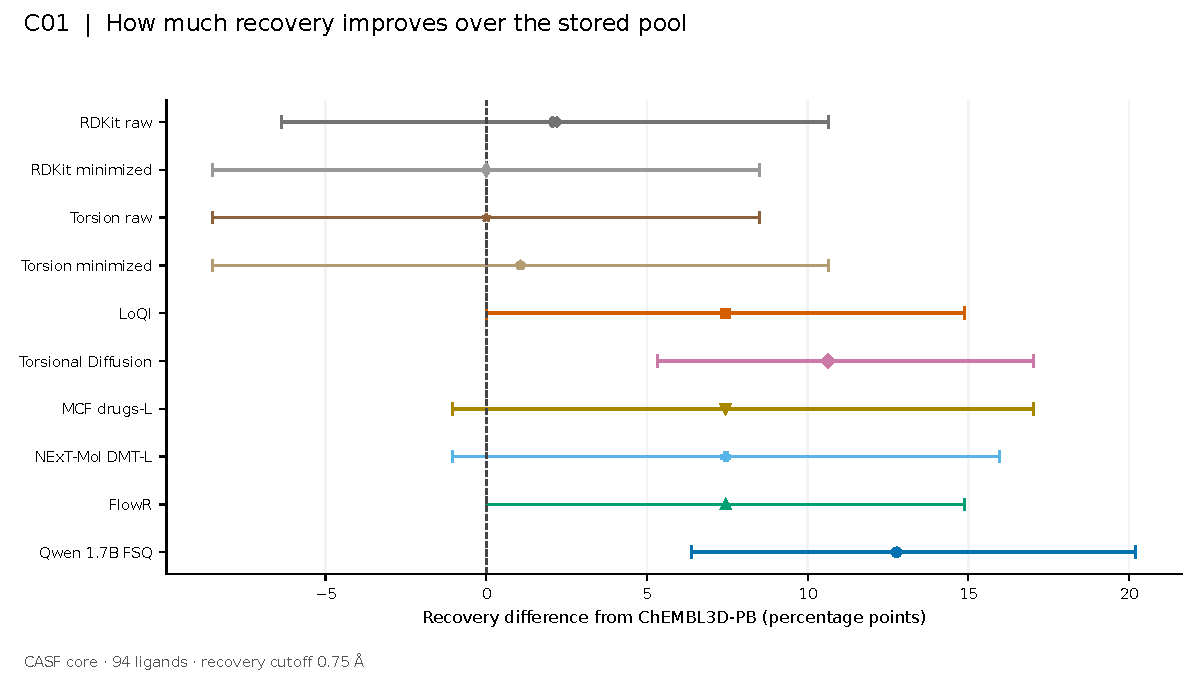
\includegraphics[width=\linewidth,height=0.72\textheight,keepaspectratio]{figures/candidates/c01-paired-recovery.pdf}
\caption{\textbf{How much recovery improves over the stored pool.} Paired differences in core recovery between each 1,000-candidate pipeline and the finite stored ChEMBL3D-PB pool. Error bars are exploratory 95\% percentile intervals from 10,000 paired bootstrap resamples of the 94 core entries (94 distinct parent compounds; seed 20260928). Missing outputs are misses. The comparison does not match retained count or computing cost, and intervals are not adjusted for multiple comparisons or checkpoint selection.}
\label{fig:candidate-c01-paired-recovery}
\end{figure}
\clearpage
\begin{figure}[p]
\centering
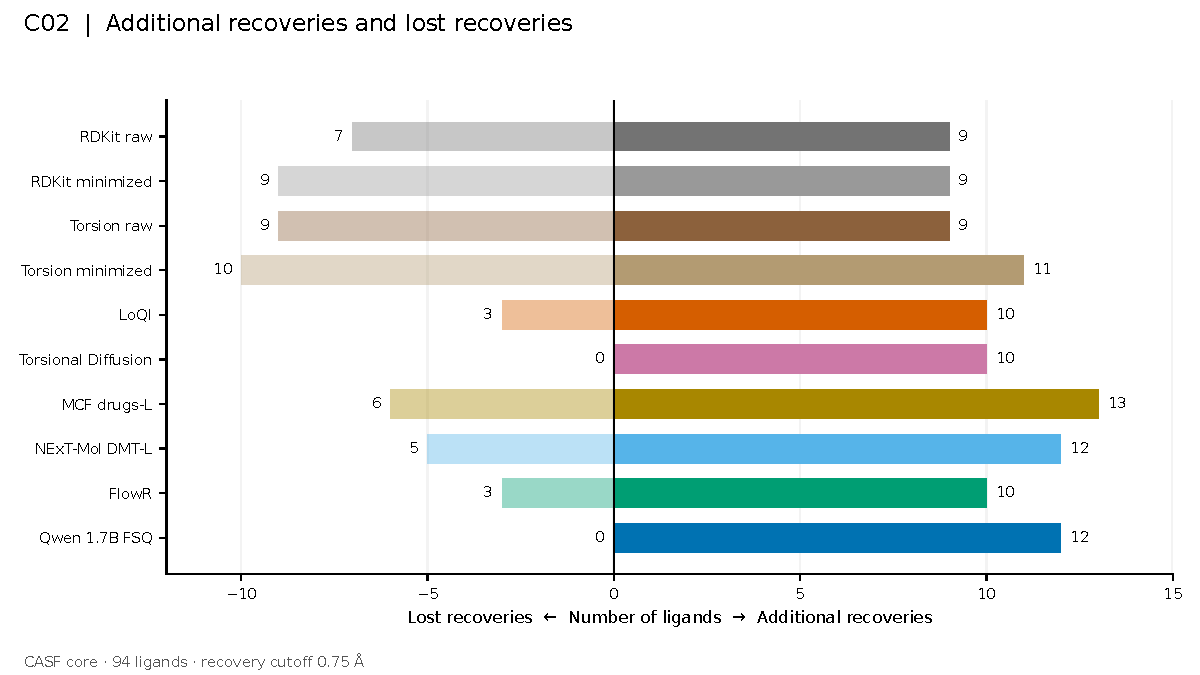
\includegraphics[width=\linewidth,height=0.72\textheight,keepaspectratio]{figures/candidates/c02-gained-lost.pdf}
\caption{\textbf{Additional recoveries and lost recoveries.} Numbers of core ligands recovered only by a generated pool (right) or only by ChEMBL3D-PB (left). Shared hits and shared misses are omitted. Generated pools use the 1,000-candidate target and PoseBusters filtering; the reference is the finite stored pool. A positive net difference need not imply improvement on every ligand.}
\label{fig:candidate-c02-gained-lost}
\end{figure}
\clearpage
\begin{figure}[p]
\centering
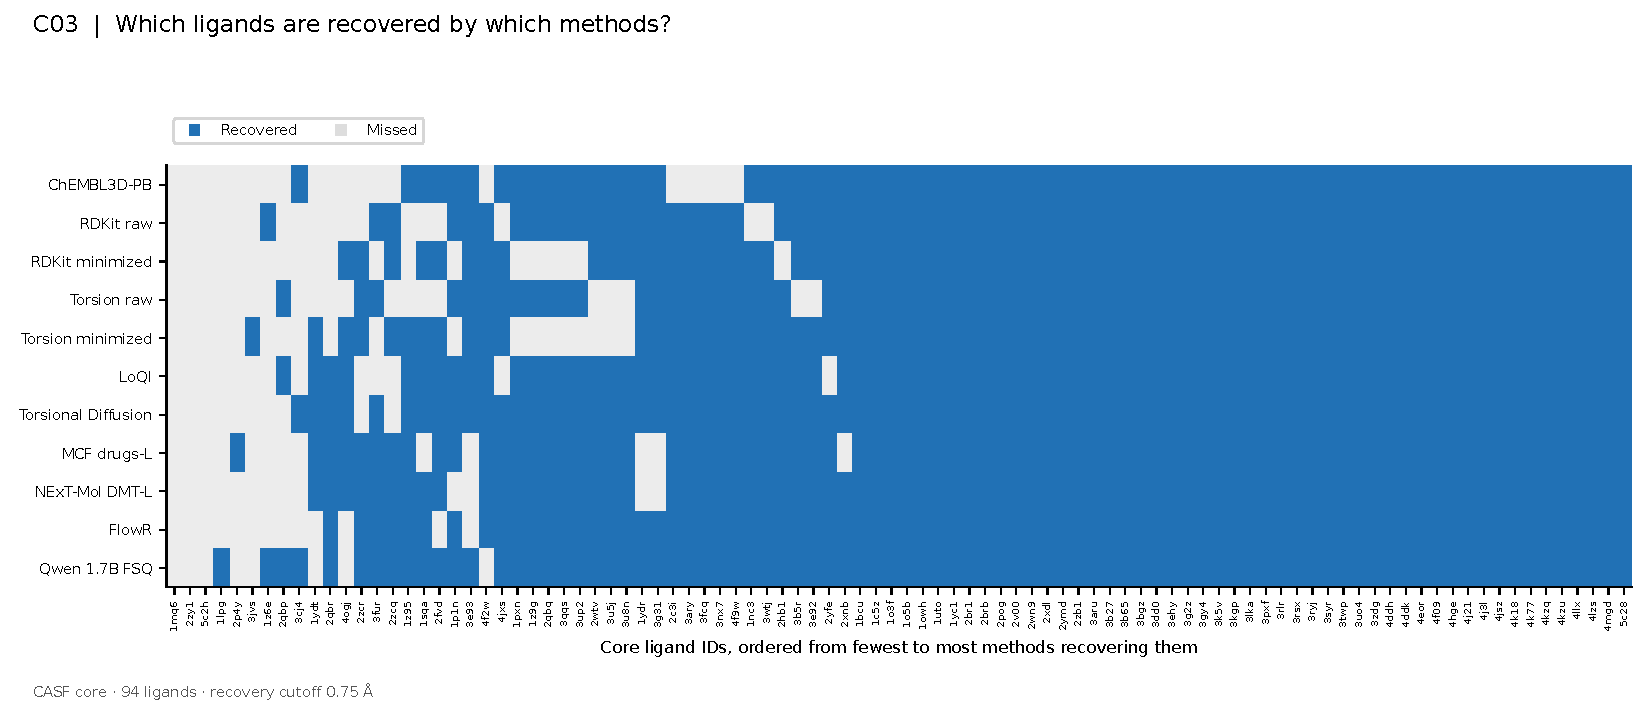
\includegraphics[width=\linewidth,height=0.72\textheight,keepaspectratio]{figures/candidates/c03-ligand-recovery.pdf}
\caption{\textbf{Which ligands are recovered by which methods?.} Binary recovery for every core ligand and each of the ten generation pipelines plus ChEMBL3D-PB. Blue cells indicate a PoseBusters-passing conformer within 0.75~\AA{}; gray cells indicate a miss, including missing output. Columns are sorted by the number of methods recovering each ligand. Generated pools use the 1,000-candidate target. This is a descriptive map of correlated outcomes, not an independent set of method trials.}
\label{fig:candidate-c03-ligand-recovery}
\end{figure}
\clearpage
\begin{figure}[p]
\centering
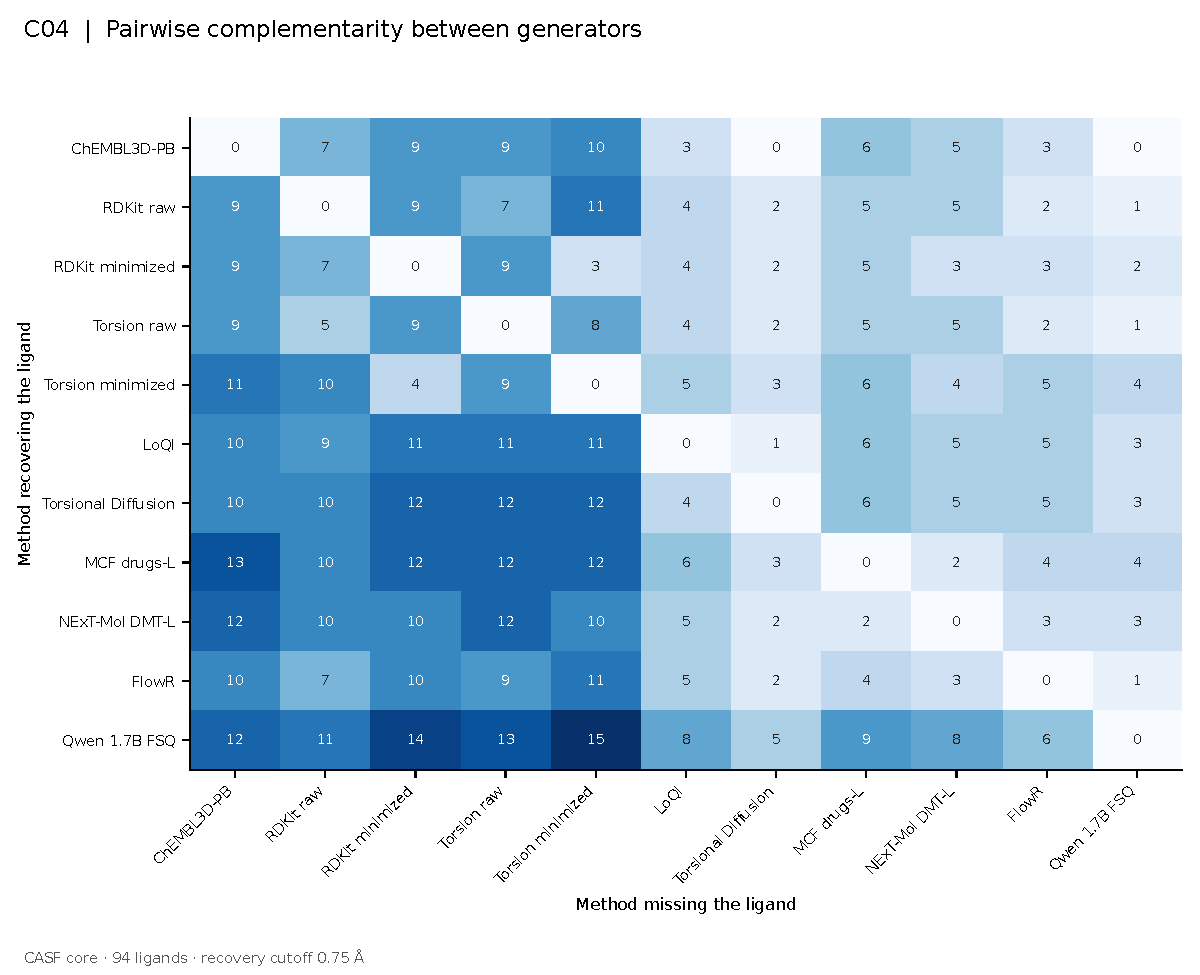
\includegraphics[width=\linewidth,height=0.72\textheight,keepaspectratio]{figures/candidates/c04-complementarity.pdf}
\caption{\textbf{Pairwise complementarity between generators.} Each cell counts ligands recovered by the row method and missed by the column method. The matrix is directional; its diagonal is zero. Generated pools use 1,000 candidates before filtering, while ChEMBL3D-PB uses its stored pool. Counts identify complementary recovery patterns; they do not measure the performance or cost of a newly generated mixed ensemble.}
\label{fig:candidate-c04-complementarity}
\end{figure}
\clearpage
\begin{figure}[p]
\centering
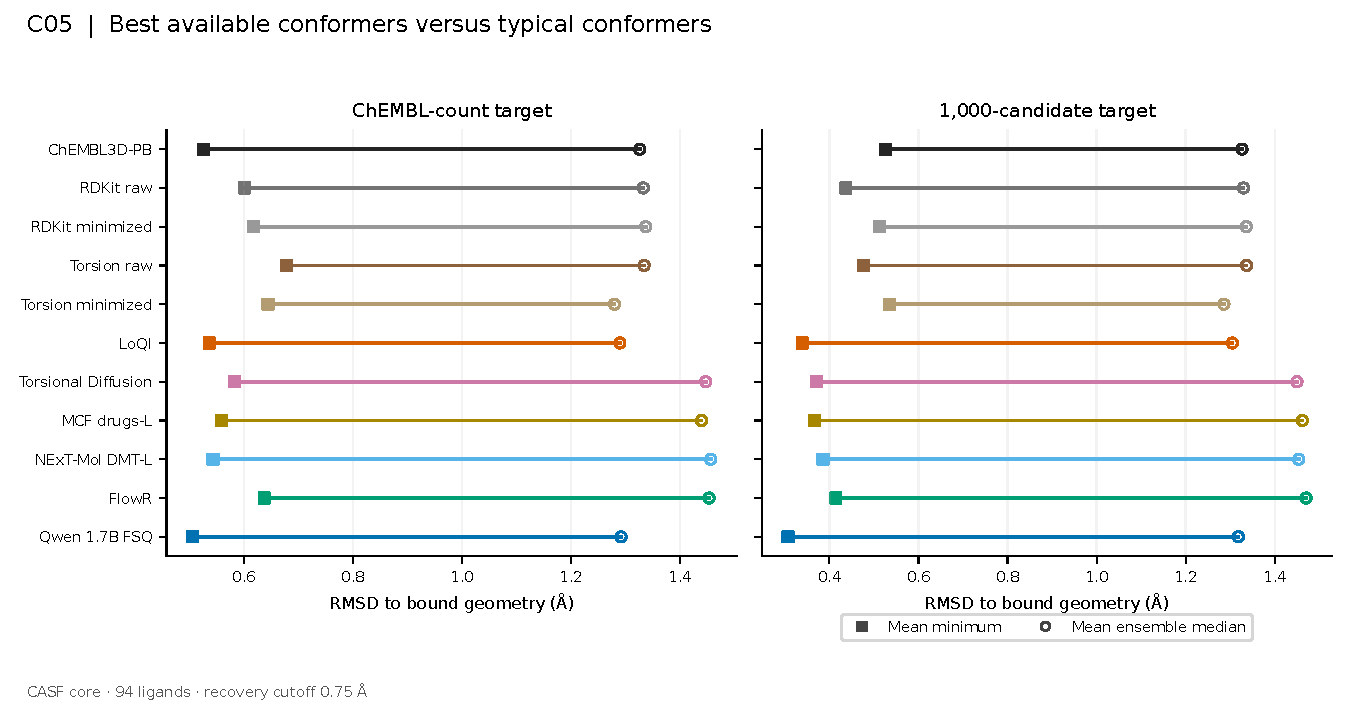
\includegraphics[width=\linewidth,height=0.72\textheight,keepaspectratio]{figures/candidates/c05-best-typical.pdf}
\caption{\textbf{Best available conformers versus typical conformers.} Mean per-ligand minimum RMSD (filled squares) and mean per-ligand ensemble-median RMSD (open circles), at both candidate targets. These continuous distances are conditional on measurable ensembles, unlike recovery fractions, whose denominator includes all 94 core entries. ChEMBL3D-PB is the same stored pool in both panels. Connecting segments indicate the difference between two summaries, not confidence intervals or paired transformations.}
\label{fig:candidate-c05-best-typical}
\end{figure}
\clearpage
\begin{figure}[p]
\centering
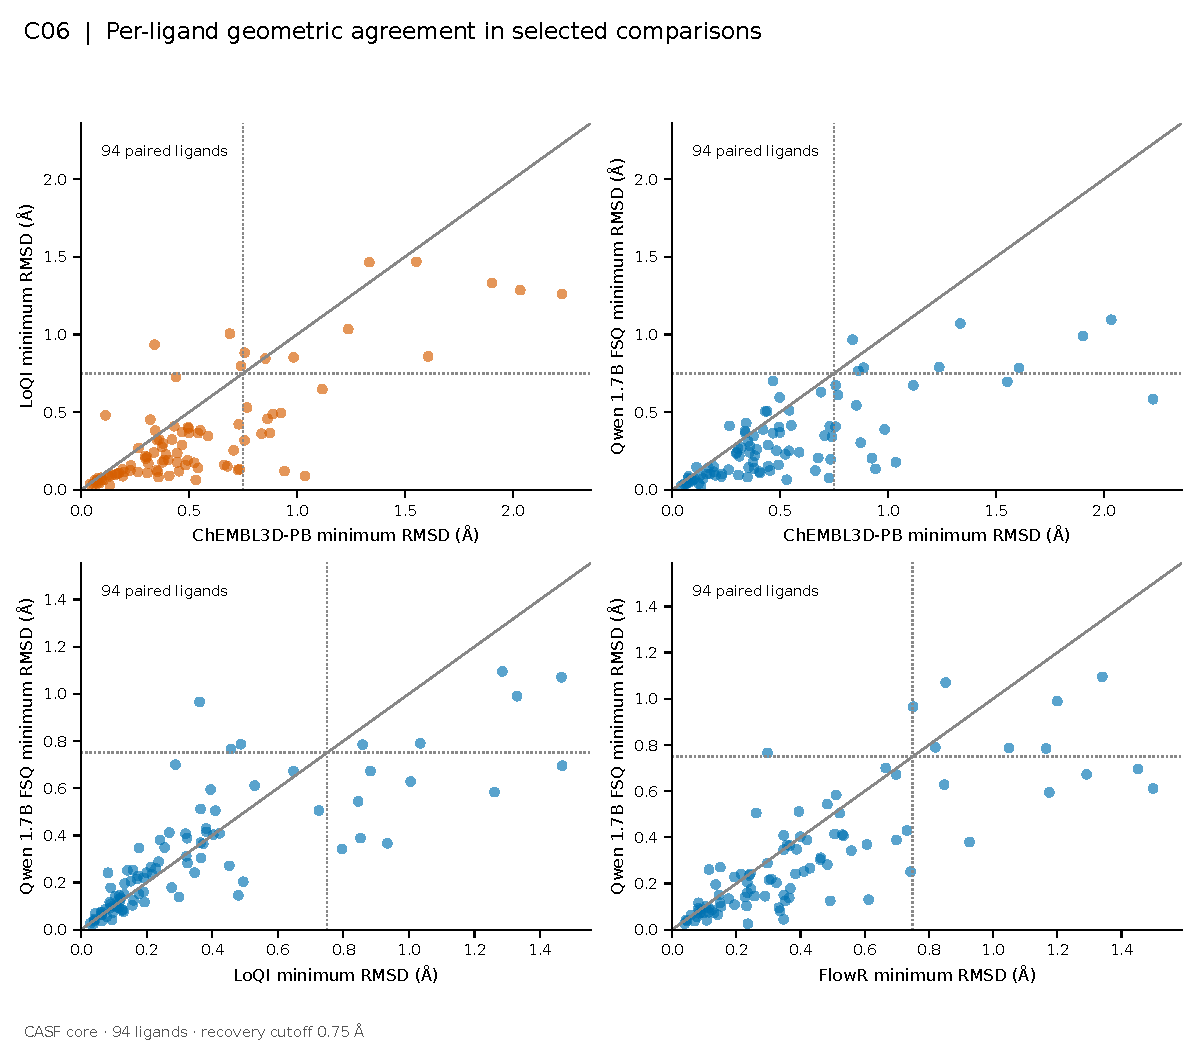
\includegraphics[width=\linewidth,height=0.72\textheight,keepaspectratio]{figures/candidates/c06-paired-rmsd.pdf}
\caption{\textbf{Per-ligand geometric agreement in selected comparisons.} Minimum RMSD for paired measurable core ensembles in four selected comparisons. Each point is one ligand; the diagonal indicates equal distance and dotted lines mark the sole recovery cutoff, 0.75~\AA{}. Lower values are better. Points below the diagonal favor the vertical-axis method. Generated pools use 1,000 candidates before filtering. Panel-specific sample counts exclude unmeasurable pairs; they are not the recovery denominator.}
\label{fig:candidate-c06-paired-rmsd}
\end{figure}
\clearpage
\begin{figure}[p]
\centering
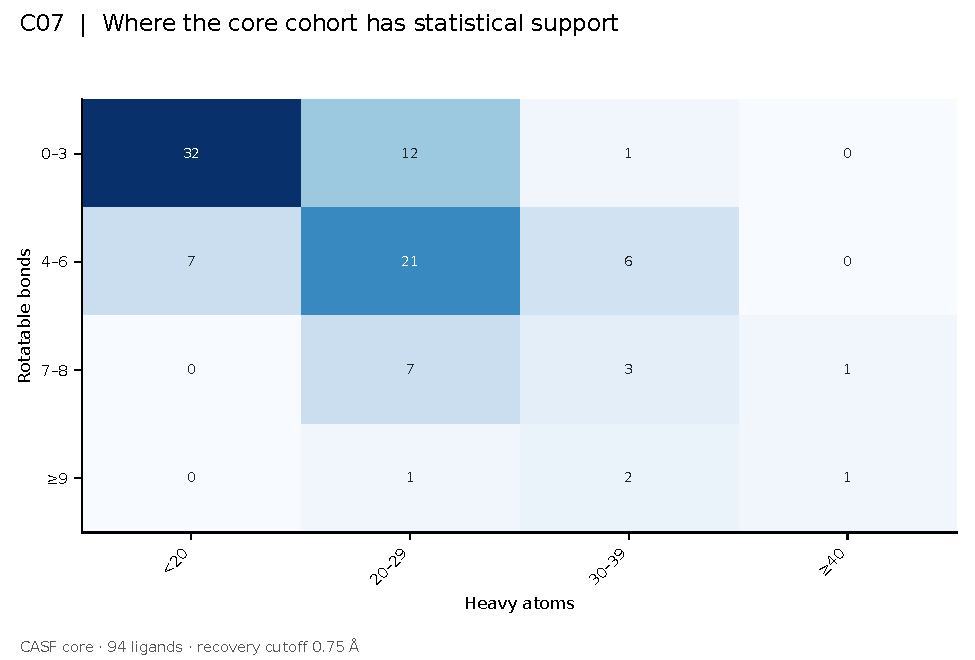
\includegraphics[width=\linewidth,height=0.72\textheight,keepaspectratio]{figures/candidates/c07-cohort-composition.pdf}
\caption{\textbf{Where the core cohort has statistical support.} Counts of the 94 core ligands cross-tabulated by heavy-atom and rotatable-bond groups using the same reference-derived descriptors for every method. Sparse large or flexible groups limit the stability of apparent method rankings. Size and flexibility are associated descriptors; this table does not isolate their independent effects.}
\label{fig:candidate-c07-cohort-composition}
\end{figure}
\clearpage
\begin{figure}[p]
\centering
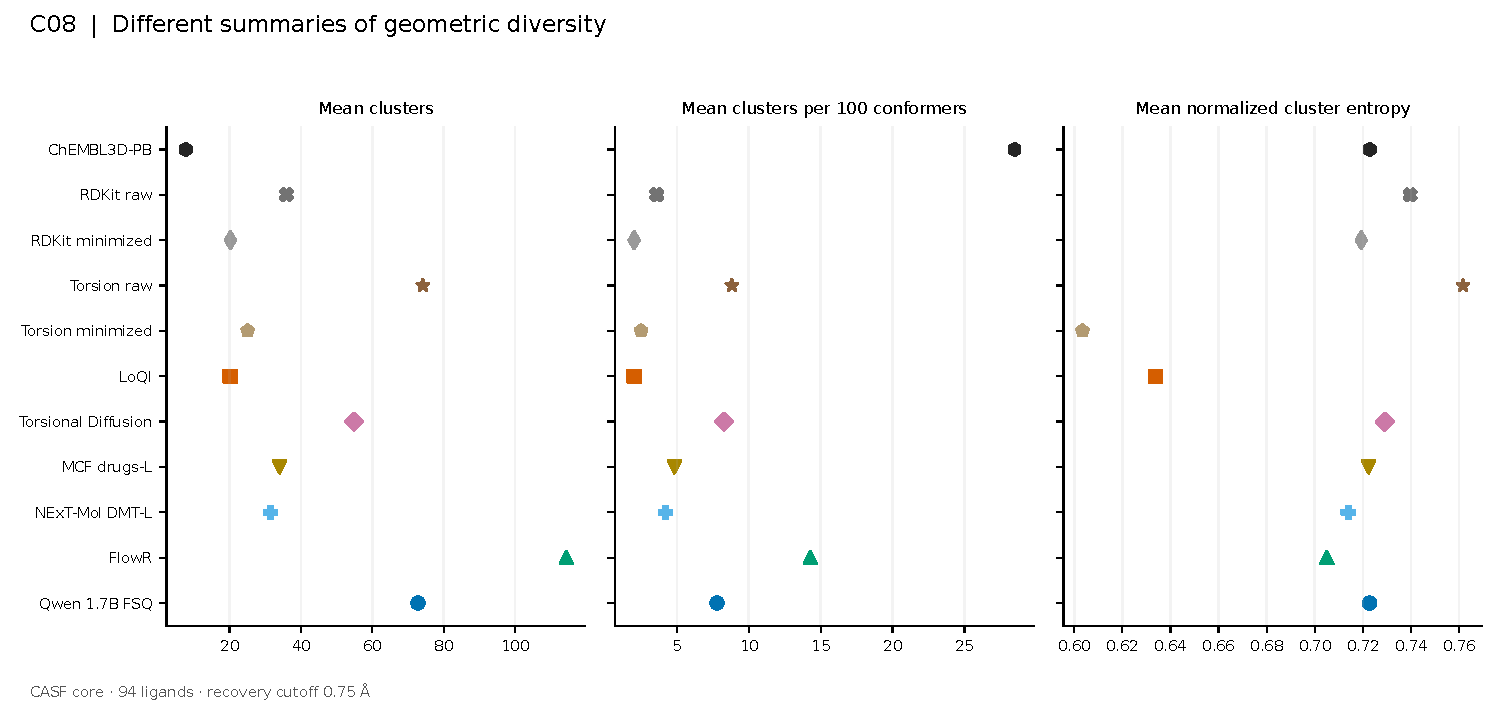
\includegraphics[width=\linewidth,height=0.72\textheight,keepaspectratio]{figures/candidates/c08-diversity-profiles.pdf}
\caption{\textbf{Different summaries of geometric diversity.} Per-ligand diversity summaries averaged over measurable core ensembles: cluster count, clusters per 100 conformers, and Shannon entropy divided by the logarithm of the number of occupied clusters (zero for a single cluster), at a 1.0~\AA{} clustering radius. This radius is distinct from the 0.75~\AA{} recovery cutoff. Generated pools use the 1,000-candidate target; ChEMBL3D-PB uses its finite pool. Normalizing cluster count does not fully remove sampling-size effects, and none of these metrics measures recovery by itself.}
\label{fig:candidate-c08-diversity-profiles}
\end{figure}
\clearpage
\begin{figure}[p]
\centering
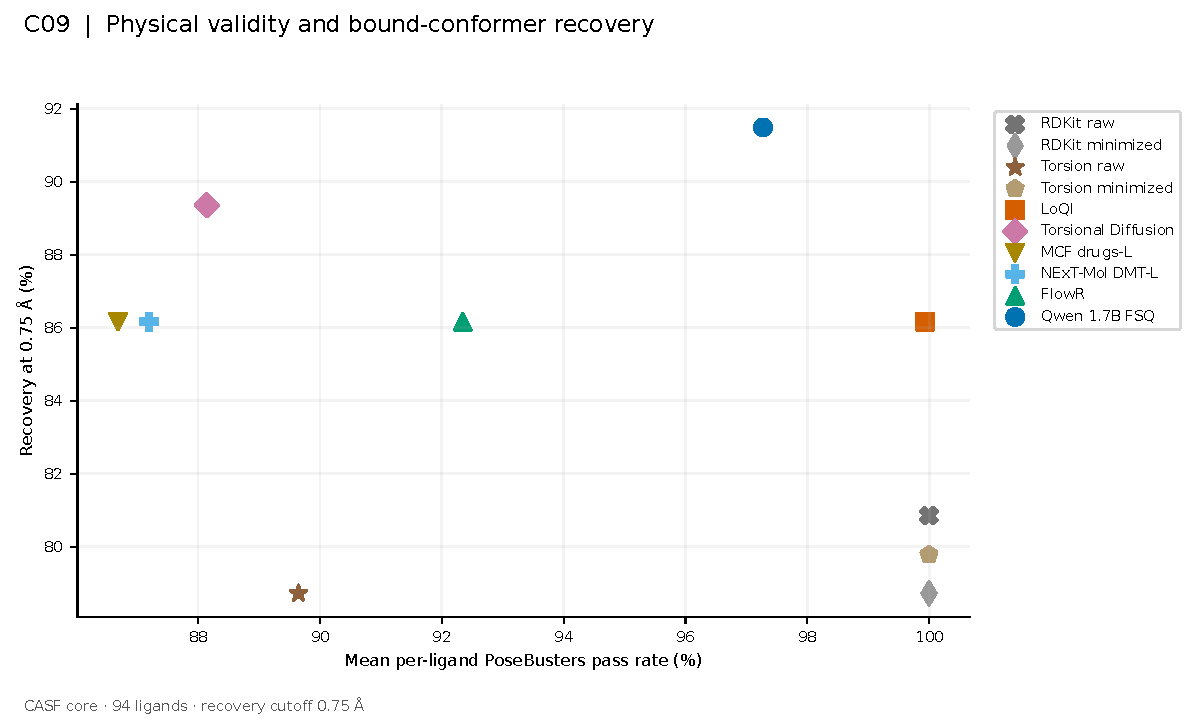
\includegraphics[width=\linewidth,height=0.72\textheight,keepaspectratio]{figures/candidates/c09-validity-recovery.pdf}
\caption{\textbf{Physical validity and bound-conformer recovery.} Mean per-ligand PoseBusters pass rate versus recovery for the ten generated core ensembles at the 1,000-candidate target. PoseBusters yield describes the analyzed input pools; it does not include every possible decoding or preprocessing rejection. Recovery requires a passing conformer and includes all 94 entries. High validity is a separate requirement from proximity to the observed bound conformation.}
\label{fig:candidate-c09-validity-recovery}
\end{figure}
\clearpage
\begin{figure}[p]
\centering
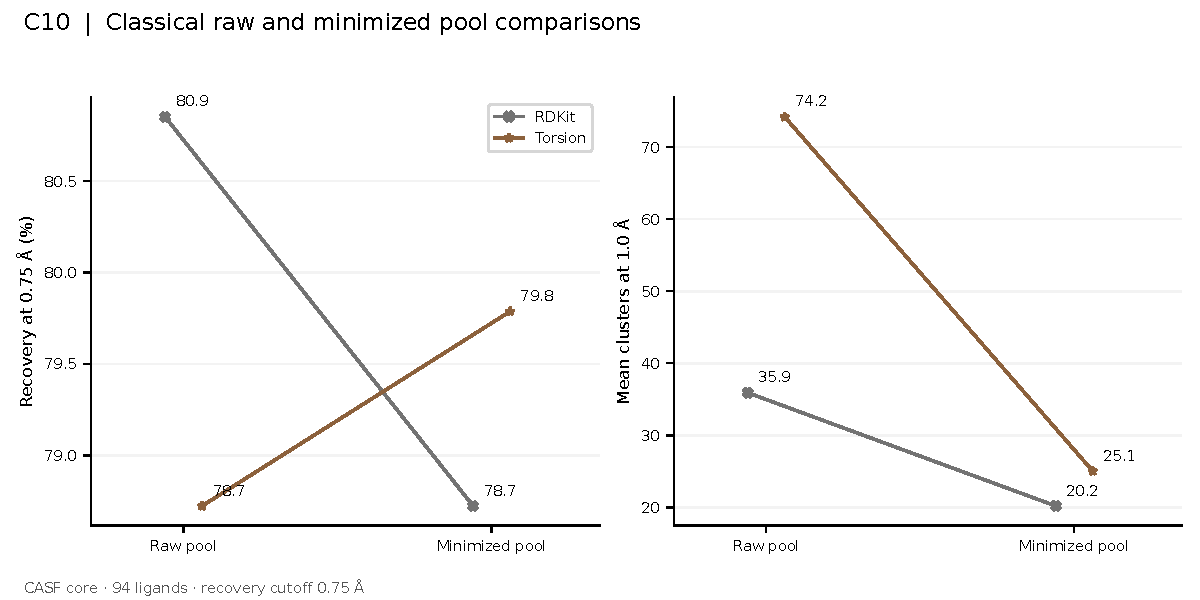
\includegraphics[width=\linewidth,height=0.72\textheight,keepaspectratio]{figures/candidates/c10-classical-pools.pdf}
\caption{\textbf{Classical raw and minimized pool comparisons.} Recovery and geometric diversity of RDKit and torsion-based raw and minimized core pools at the 1,000-candidate target. These are separately generated endpoint pools, not paired before-and-after measurements on identical conformers. Lines identify related pipelines and do not establish a causal effect of minimization. Diversity is averaged over measurable ensembles; recovery includes all core ligands.}
\label{fig:candidate-c10-classical-pools}
\end{figure}
\clearpage
\begin{figure}[p]
\centering
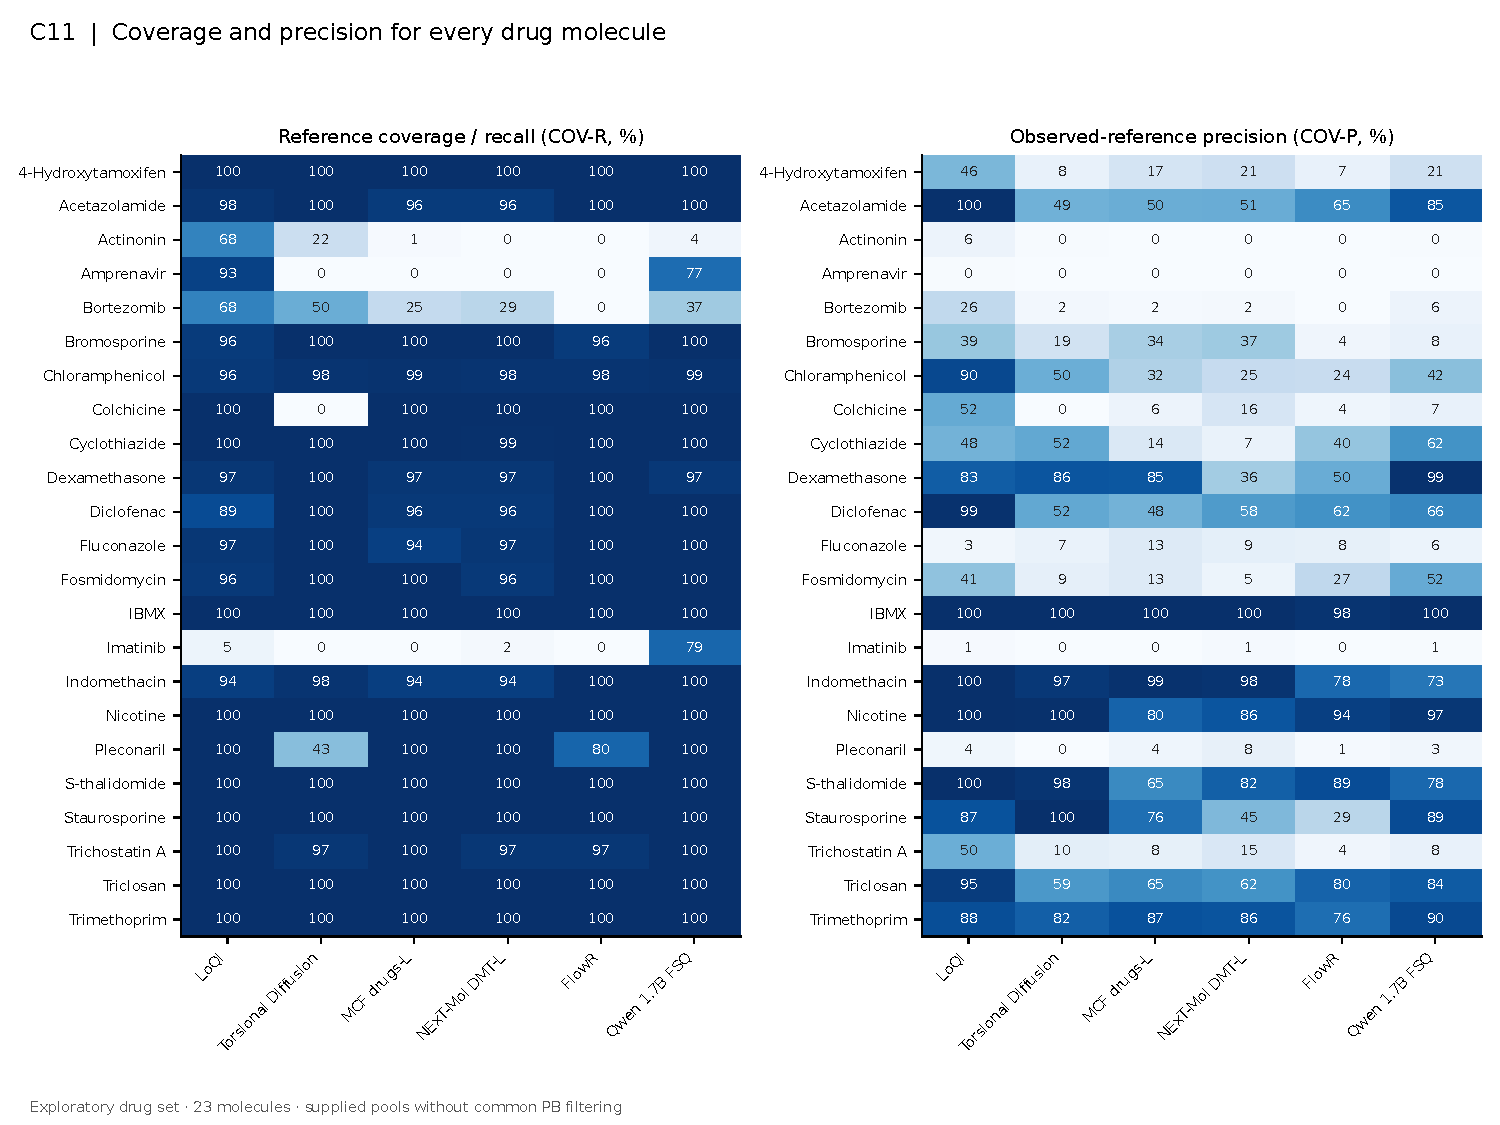
\includegraphics[width=\linewidth,height=0.72\textheight,keepaspectratio]{figures/candidates/c11-drug-coverage-matrix.pdf}
\caption{\textbf{Coverage and precision for every drug molecule.} Molecule-level COV-R and COV-P at the strict 0.75~\AA{} cutoff for all six selected generators. The two panels share a 0--100\% color scale. COV-R measures the fraction of observed references reached; COV-P measures the fraction of generated conformers near an observed reference. Unmatched conformers are not necessarily biologically impossible. All drug metrics describe supplied pools without a common PoseBusters mask; failed-RMSD handling also differs between imported evaluations. These are exploratory comparisons.}
\label{fig:candidate-c11-drug-coverage-matrix}
\end{figure}
\clearpage
\begin{figure}[p]
\centering
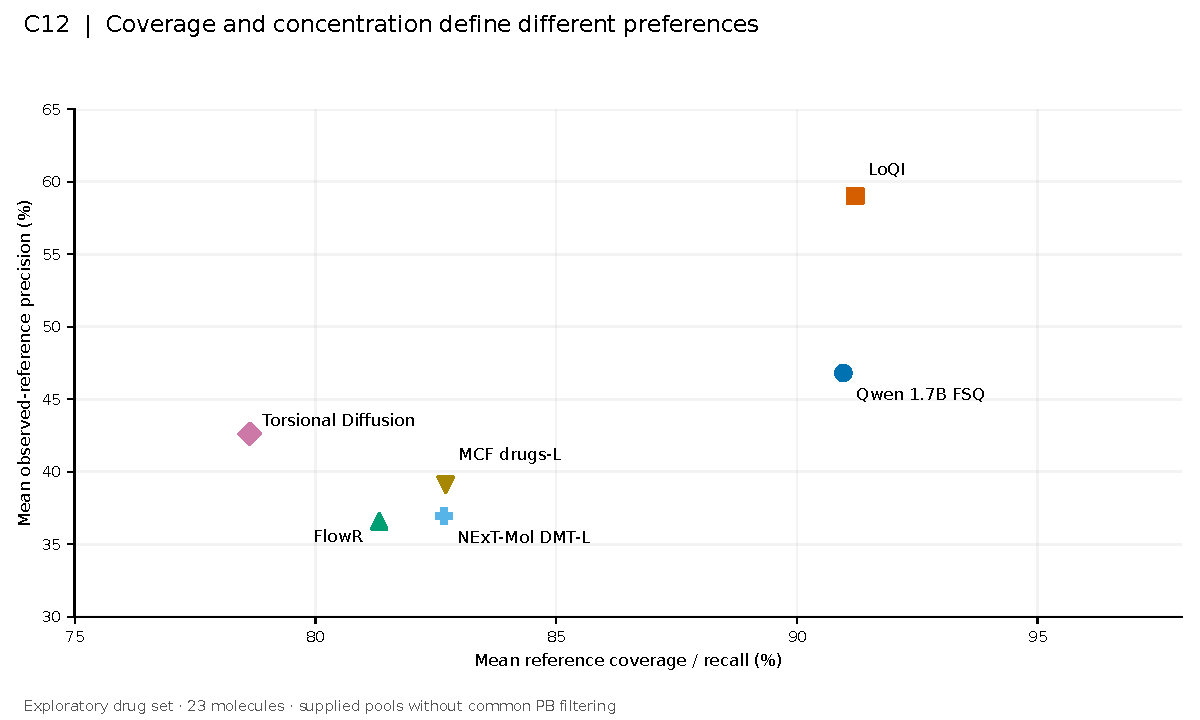
\includegraphics[width=\linewidth,height=0.72\textheight,keepaspectratio]{figures/candidates/c12-drug-tradeoff.pdf}
\caption{\textbf{Coverage and concentration define different preferences.} Molecule-mean recall and precision at 0.75~\AA{} for the six selected generators. Each of the 23 molecules receives equal weight regardless of its reference count. Higher values indicate broader observed-reference coverage or greater concentration near the available observations; they do not measure binding affinity or conformer populations. All drug metrics describe supplied pools without a common PoseBusters mask; failed-RMSD handling also differs between imported evaluations. These are exploratory comparisons.}
\label{fig:candidate-c12-drug-tradeoff}
\end{figure}
\clearpage
\begin{figure}[p]
\centering
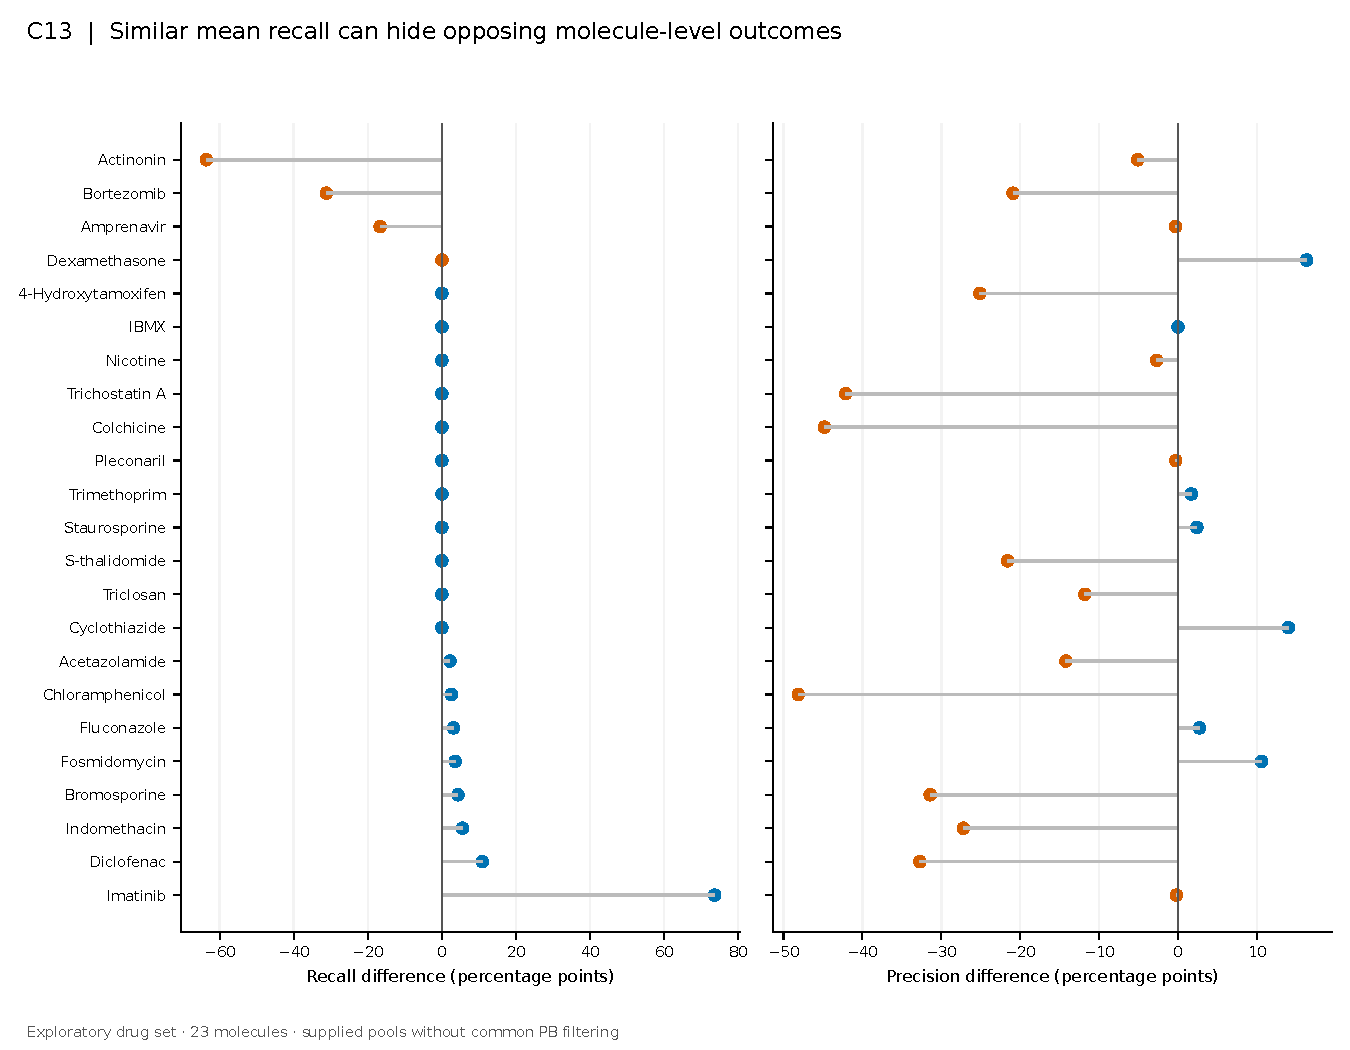
\includegraphics[width=\linewidth,height=0.72\textheight,keepaspectratio]{figures/candidates/c13-drug-paired-molecules.pdf}
\caption{\textbf{Similar mean recall can hide opposing molecule-level outcomes.} Paired molecule-level differences, Qwen 1.7B FSQ minus LoQI, in recall and precision at 0.75~\AA{}. Molecules are sorted by the recall difference and retain that ordering in both panels. Positive values favor Qwen, negative values favor LoQI. These descriptive differences are not per-molecule confidence intervals. All drug metrics describe supplied pools without a common PoseBusters mask; failed-RMSD handling also differs between imported evaluations. These are exploratory comparisons.}
\label{fig:candidate-c13-drug-paired-molecules}
\end{figure}
\clearpage
\begin{figure}[p]
\centering
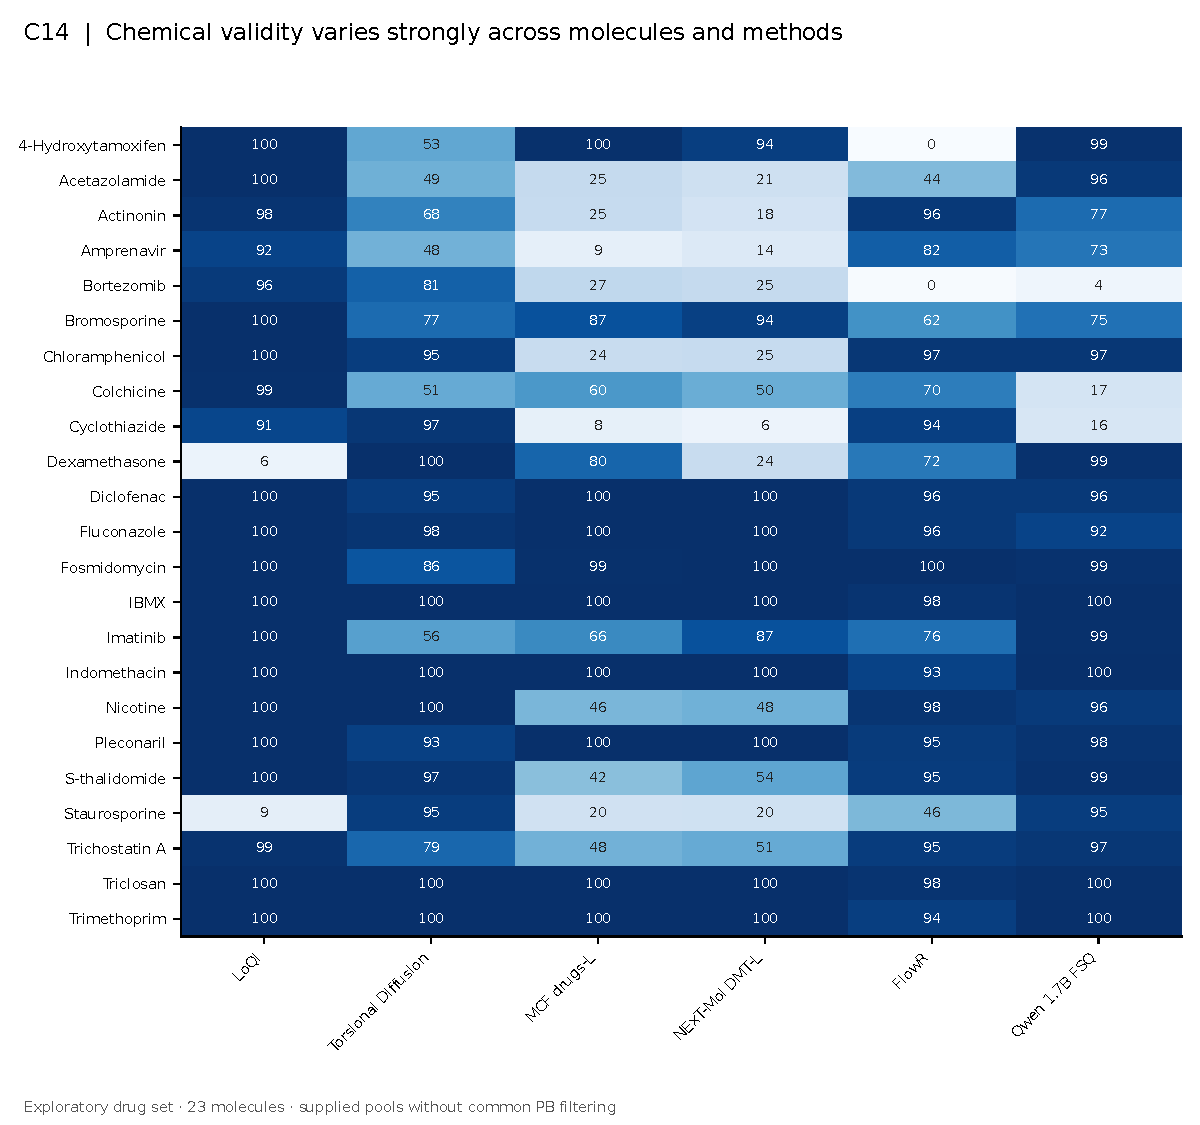
\includegraphics[width=\linewidth,height=0.72\textheight,keepaspectratio]{figures/candidates/c14-drug-validity.pdf}
\caption{\textbf{Chemical validity varies strongly across molecules and methods.} PoseBusters pass percentages for each supplied drug molecule--method pool. The common color scale spans 0--100\%. Validity is reported separately from coverage and precision: coverage cannot be adjusted by multiplying it by these percentages because the passing conformers and recovered references need not coincide. All drug metrics describe supplied pools without a common PoseBusters mask; failed-RMSD handling also differs between imported evaluations. These are exploratory comparisons.}
\label{fig:candidate-c14-drug-validity}
\end{figure}
\clearpage
\begin{figure}[p]
\centering
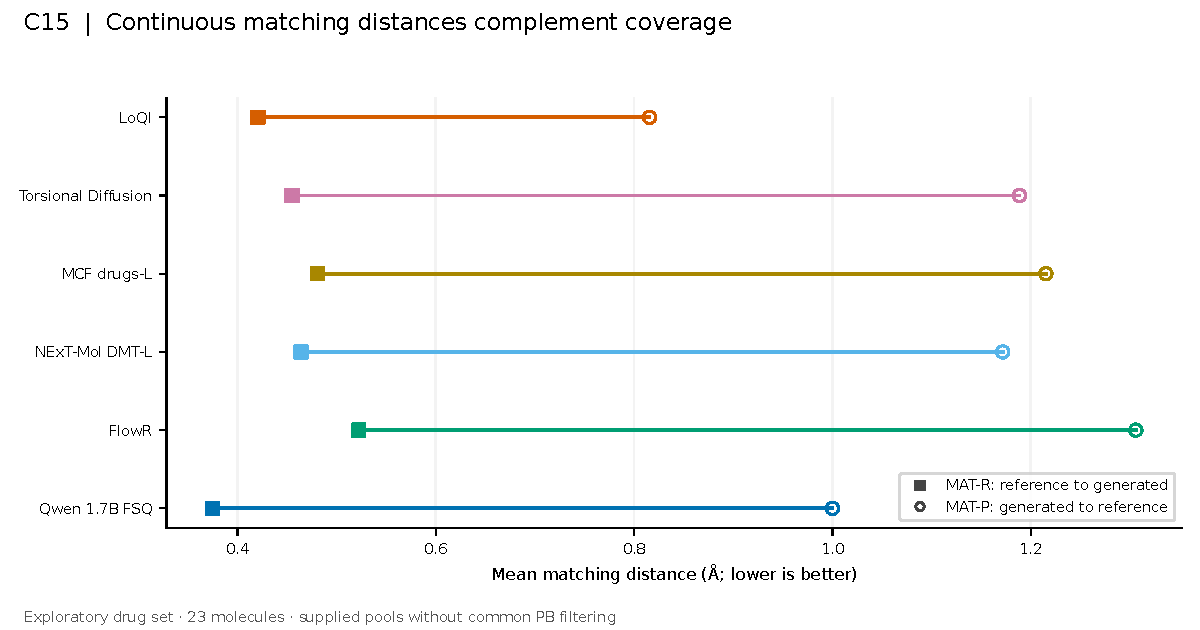
\includegraphics[width=\linewidth,height=0.72\textheight,keepaspectratio]{figures/candidates/c15-drug-matching-distance.pdf}
\caption{\textbf{Continuous matching distances complement coverage.} Molecule-mean MAT-R and MAT-P for the six selected generators. MAT-R averages nearest generated-conformer distances from observed references; MAT-P averages nearest observed-reference distances from generated conformers. Lower is better. Segments connect distinct summaries rather than uncertainty bounds. All drug metrics describe supplied pools without a common PoseBusters mask; failed-RMSD handling also differs between imported evaluations. These are exploratory comparisons.}
\label{fig:candidate-c15-drug-matching-distance}
\end{figure}
\clearpage
\begin{figure}[p]
\centering
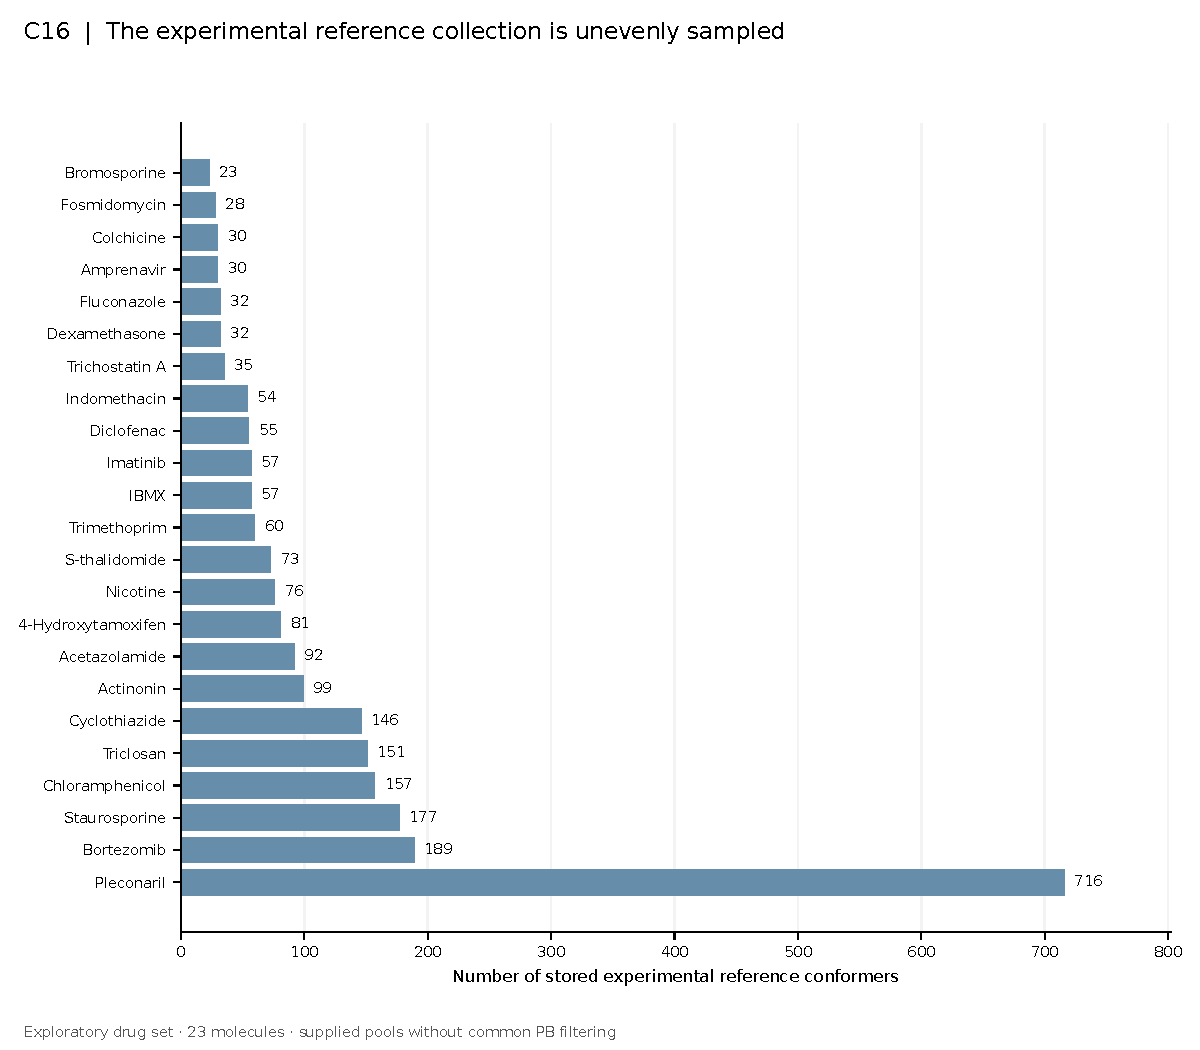
\includegraphics[width=\linewidth,height=0.72\textheight,keepaspectratio]{figures/candidates/c16-drug-reference-counts.pdf}
\caption{\textbf{The experimental reference collection is unevenly sampled.} Numbers of stored experimental reference conformers for the 23 drug molecules (2,450 in total). Reference counts are not counts of unique conformational states: redundant or very similar geometries may recur. Reported coverage and precision aggregates average molecules equally, so reference-rich molecules do not receive extra aggregate weight.}
\label{fig:candidate-c16-drug-reference-counts}
\end{figure}
\clearpage
\begin{figure}[p]
\centering
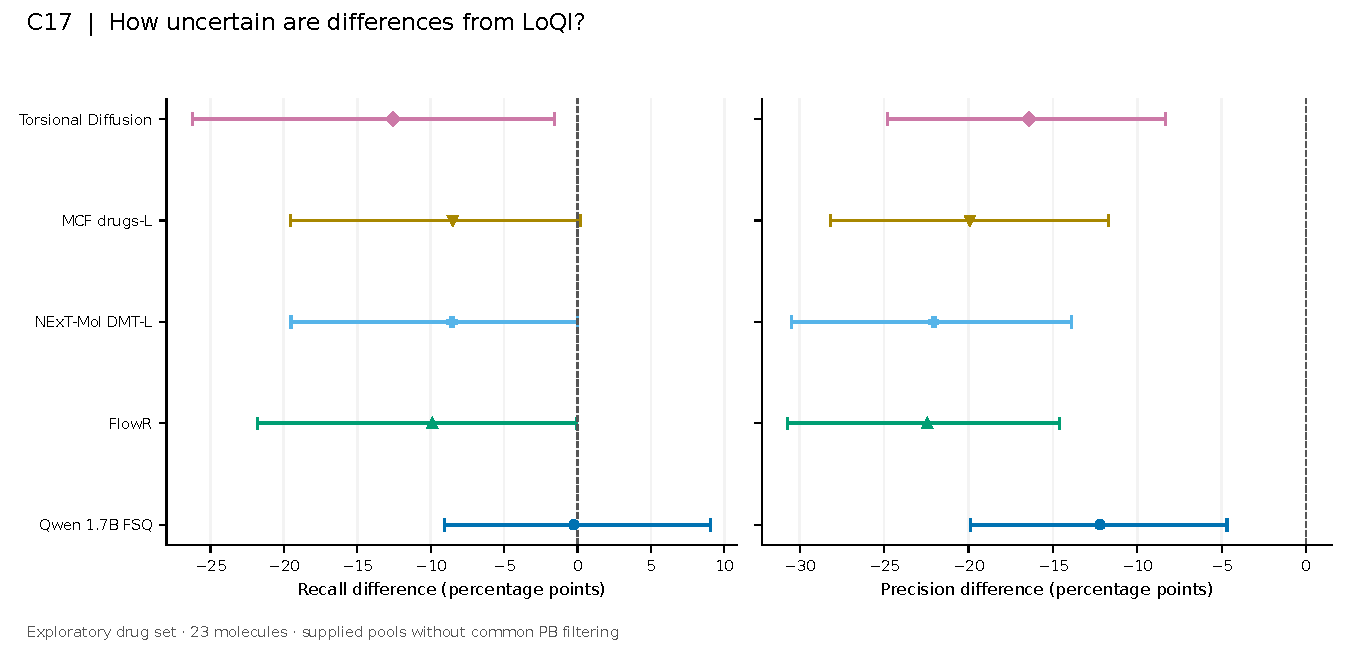
\includegraphics[width=\linewidth,height=0.72\textheight,keepaspectratio]{figures/candidates/c17-drug-paired-uncertainty.pdf}
\caption{\textbf{How uncertain are differences from LoQI?.} Paired differences from LoQI in molecule-mean COV-R and COV-P at 0.75~\AA{}. Error bars are exploratory 95\% percentile intervals from 10,000 paired molecule bootstrap samples (23 molecules; seed 20260928). These newly rendered intervals can differ slightly from earlier exports because the resampling seed differs. Intervals are not adjusted for multiple comparisons; an interval crossing zero does not establish equivalence. All drug metrics describe supplied pools without a common PoseBusters mask; failed-RMSD handling also differs between imported evaluations. These are exploratory comparisons.}
\label{fig:candidate-c17-drug-paired-uncertainty}
\end{figure}
\clearpage
\begin{figure}[p]
\centering
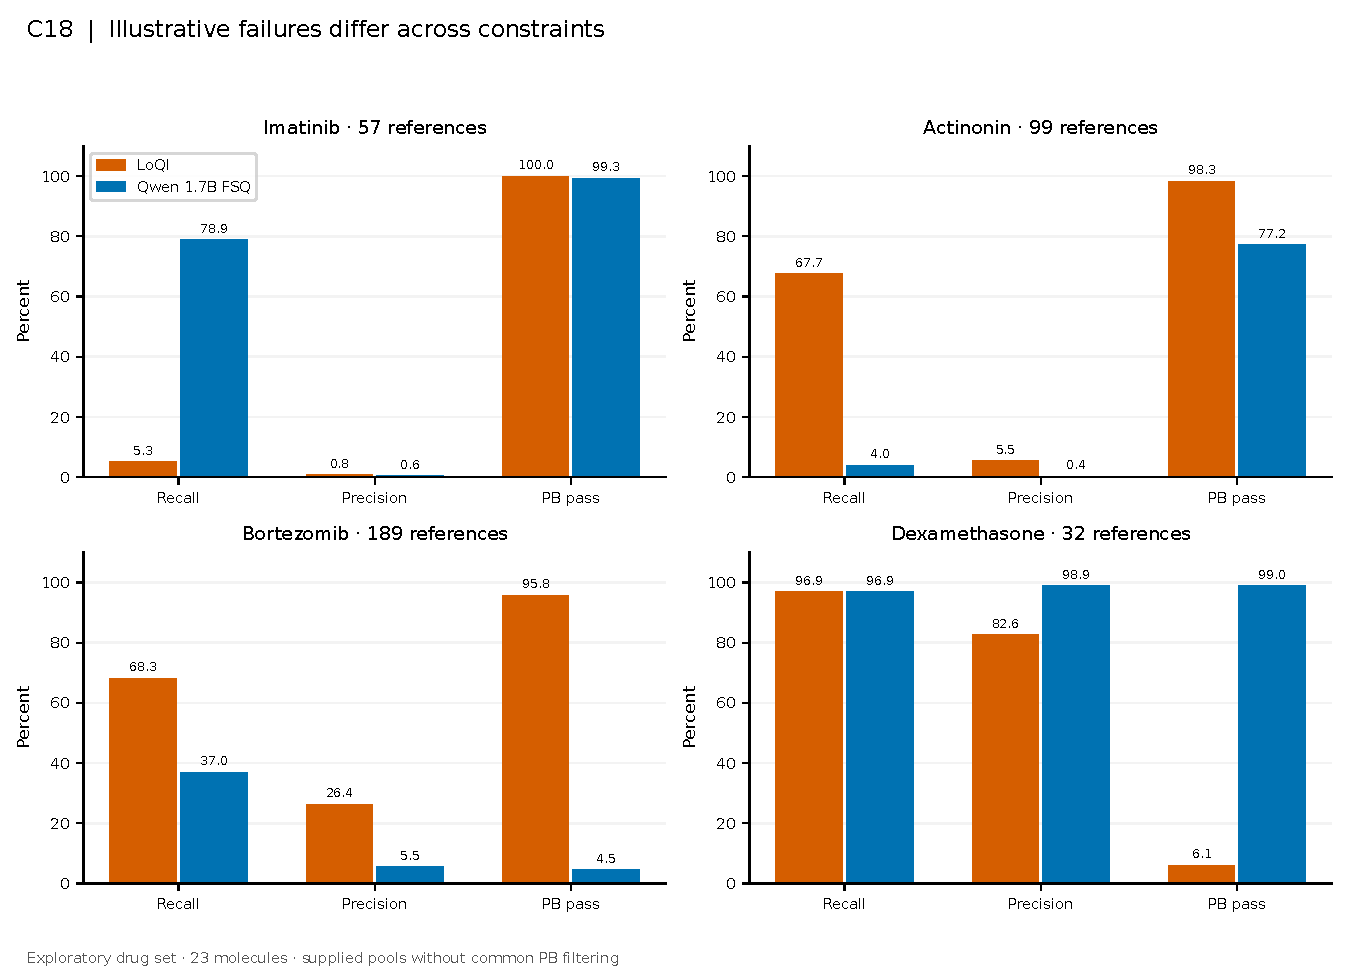
\includegraphics[width=\linewidth,height=0.72\textheight,keepaspectratio]{figures/candidates/c18-drug-case-profiles.pdf}
\caption{\textbf{Illustrative failures differ across constraints.} Four post hoc illustrative molecules comparing LoQI and Qwen 1.7B FSQ: recall, precision, and PoseBusters pass rate. Coverage uses the strict 0.75~\AA{} cutoff. The cases illustrate opposing recall preferences and disagreements between geometric coverage and chemical validity; they are not a representative sample or a structural explanation. All drug metrics describe supplied pools without a common PoseBusters mask; failed-RMSD handling also differs between imported evaluations. These are exploratory comparisons.}
\label{fig:candidate-c18-drug-case-profiles}
\end{figure}
\clearpage
\endgroup


\end{document}
